\chapter
%[Finding Optimal Sequences for Area Aggregation]
{Finding Optimal Sequences for Area Aggregation~-- \\
	\Astar vs.\ Integer Linear Programming}
\label{chap:AreaAgg}




%\todo[inline]{review paper \cite{haunertwolff2010}}


A \emph{land-cover map} is a planar subdivision in which each 
area belongs to a
land-cover class or \emph{type}.
Suppose that there are two land-cover maps of 
different scales 
that cover the same spatial region.
We consider the problem of finding a sequence 
of small incremental changes 
that gradually transforms 
the larger-scale map (the \emph{start map}) to 
the smaller-scale map (the \emph{goal map}).
We use this sequence to generate and show land-cover maps at 
intermediate scales (see \fig\ref{fig:AreaAgg_example}).
In this way, we can avoid large and sudden changes 
that distract users 
when they are zooming in or out.

With the same motivation, a strategy of hierarchical schemes 
has been proposed.
This strategy generalizes a more-detailed representation 
to obtain a less-detailed representation 
based on small incremental changes, 
e.g., the Generalized Area Partitioning tree 
(GAP-tree),
which can be constructed if only the larger-scale map is given
\citep{vanOosterom1995Development} 
or if both the larger-scale map and the smaller-scale map 
are given \citep{HaunertDilo2009}. 

Typically, the next change in such a sequence 
is determined locally, 
in a greedy fashion.  
If we insist on finding a sequence that is, 
according to some global measure, optimal, 
the problem becomes complicated.

\begin{figure}[tb]
	\centering
	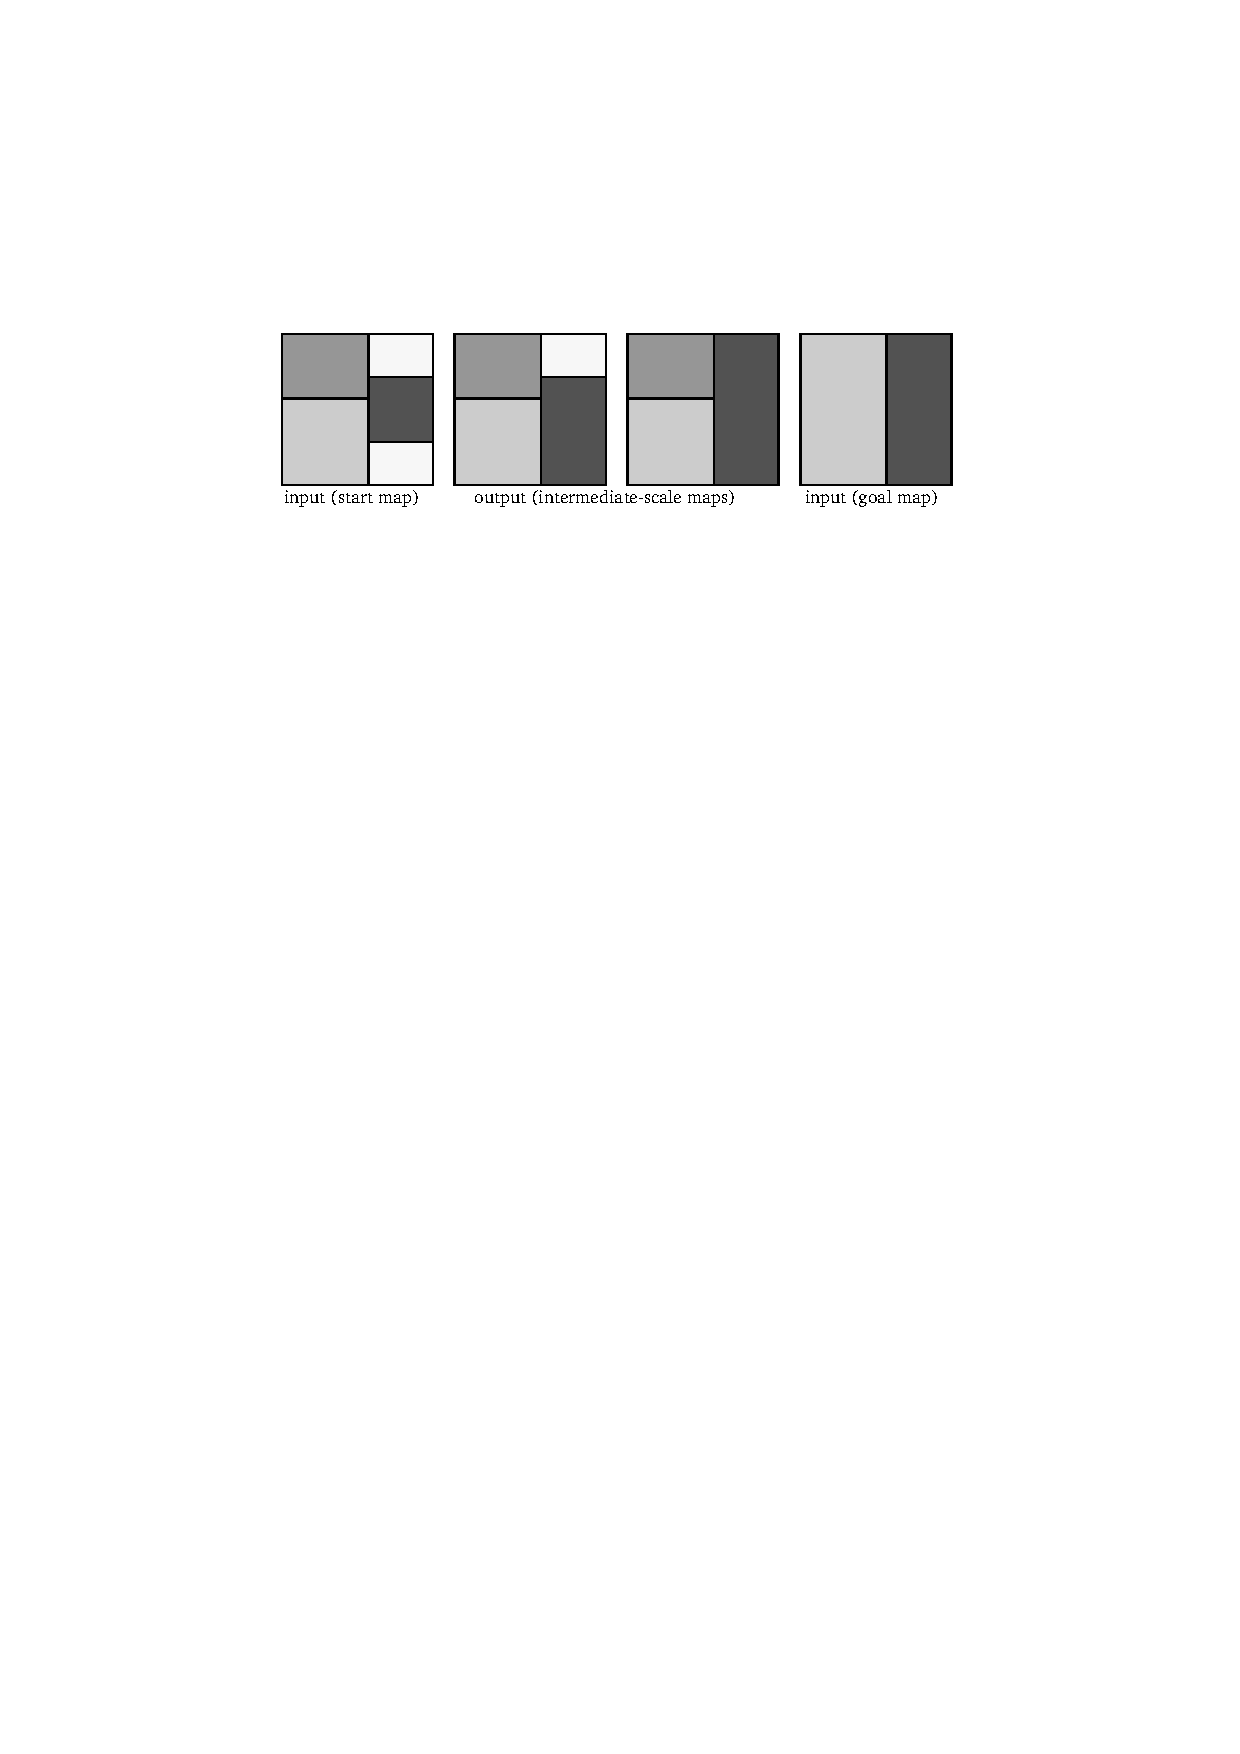
\includegraphics{AreaAgg_example}
	\caption{The input and a possible output for an instance of 
	our problem}
	\label{fig:AreaAgg_example}
\end{figure}

We assume that there exist many-to-one relationships between the 
areas of the
start map and the areas of the goal map.
\revise{}{This assumption is based on the fact that there are 
many algorithms 
	\citep[e.g.,][]{HaunertWolff2010AreaAgg, vanSmaalen2003, 
		Cheng2006} that aggregate 
	some land-cover areas into one single land-cover area. The 
	input and the 
	generalized results of these methods can be used as our 
	input.}
\revise{(which we term \emph{regions}).}{We term the areas of 
the goal map 
	\emph{regions}.} 
That is, every region is the union of a set of areas 
\revise{in}{on} the start map.

The type of a region may differ from the types of its 
components. 
For example, a small water area together with 
multiple adjacent forest areas may constitute 
a large forest region in the smaller scale.
We assume, however, that every region, on goal map, 
contains at least one area of the same type on start map.
Our assumptions hold if the goal map has been produced 
with an automatic method for area aggregation, 
for example, with the method of \citet{HaunertWolff2010AreaAgg}.
That method produces a land-cover map at a single output scale, 
given a land-cover map at a larger scale.
It is based on global optimization and minimizes 
type changes as well as a cost for non-compact shapes 
while satisfying constraints on the sizes of the output regions.
Although \textcite{HaunertWolff2010AreaAgg}
leads to results of high quality, 
it does not yield land-cover maps at intermediate scales.

\todo[inline]{more research work about generalization of land 
cover maps}

To generate a good sequence of maps, 
we must consider the sequence of maps as a whole 
instead of considering each intermediate-scale map independently.
On the other hand, to simplify the problem,
we first consider each region of the goal map 
(with its components on the start map) 
independent of the other regions.
Once we have found an aggregation sequence of maps for each region, 
we integrate all the sequences into an overall sequence 
that transforms the start map into the goal map. 
Our aggregation sequence may be stored in data structures
such as the GAP-face tree \citep{vanOosterom2005} 
or the map cube model \citep{Timpf1998} 
to support on-the-fly display.


\mypar{Contribution}
We give general ideas and basic concepts of our method, 
and analyze the size of our problem (see 
\sect\ref{sec:AreaAgg_Preliminaries}).

We present a new global optimization approach to solve this 
problem. 
Our approach is based on the \Astar algorithm 
(see \sect\ref{sec:AreaAgg_AStar}) 
which handles the combinatorial explosion that 
we will discuss in \sect\ref{sec:AreaAgg_Preliminaries}.
We also present an alternative approach via integer linear
programming.  That is, we model our problem as a integer linear
program (ILP) using variables, constraints, and an objective
function.  In an ILP, the constraints and the objective function must
be \emph{linear} in the variables, which makes it difficult to express
requirements such as the compactness of areas.  Other than in a linear
program (LP), we can use binary (0--1) variables, which helps us to
model our problem, but in general, it is NP-hard to solve an ILP
optimally.  

We define our cost functions in \sect\ref{sec:AreaAgg_CostFunctions}.
We compare three methods for finding aggregation sequences, namely,
\Astar (\sect\ref{sec:AreaAgg_AStar}), 
an ILP-based algorithm (\sect\ref{sec:AreaAgg_ILP}), and
a greedy algorithm (\sect\ref{sec:AreaAgg_Greedy}), 
By comparing with the greedy algorithm, 
which is used as a benchmark,
we are able to see if it is worth 
to use \Astar or the ILP-based algorithm, 
which are more complex and slower.  Our case study 
uses a dataset of the German topographic database ATKIS 
(see \sect\ref{sec:AreaAgg_CaseStudy}).  

We do not deal with the simplification of lines in this chapter, 
since this can be handled separately from the
aggregation of areas, for example, 
by using the method of \citet{Douglas1973} 
or \citet{Saalfeld1999}.
Those methods can be used to set up 
the binary line generalization tree (BLG-tree)
\citep{vanOosterom1995Development},
which is a hierarchical data structure that 
defines a gradual line simplification process.

We conclude this chapter in \sect\ref{sec:AreaAgg_Conclusions}.

\section{Preliminaries}
\label{sec:AreaAgg_Preliminaries}


To allow us to describe our method more easily,
we assume that the goal map has only one region. 
On the start map, the same region consists of~$n$ land-cover 
areas (components). 
In other words, the union of the $n$ land-cover areas 
is the only region on the goal map.  
We show how to compute an aggregation sequence for a region. 
For a goal map with more than one region, 
we ``interleaf'' aggregation sequences of different regions
with respect to the order of the smallest patches 
(see for example \fig\ref{fig:AreaAgg_IntegrateSequence}).
This integration is similar to the merge step in the 
sorting algorithm Mergesort; 
see \textcite[pp.~29--37]{Cormen2009}.
\begin{figure*}[tb]
	\centering
	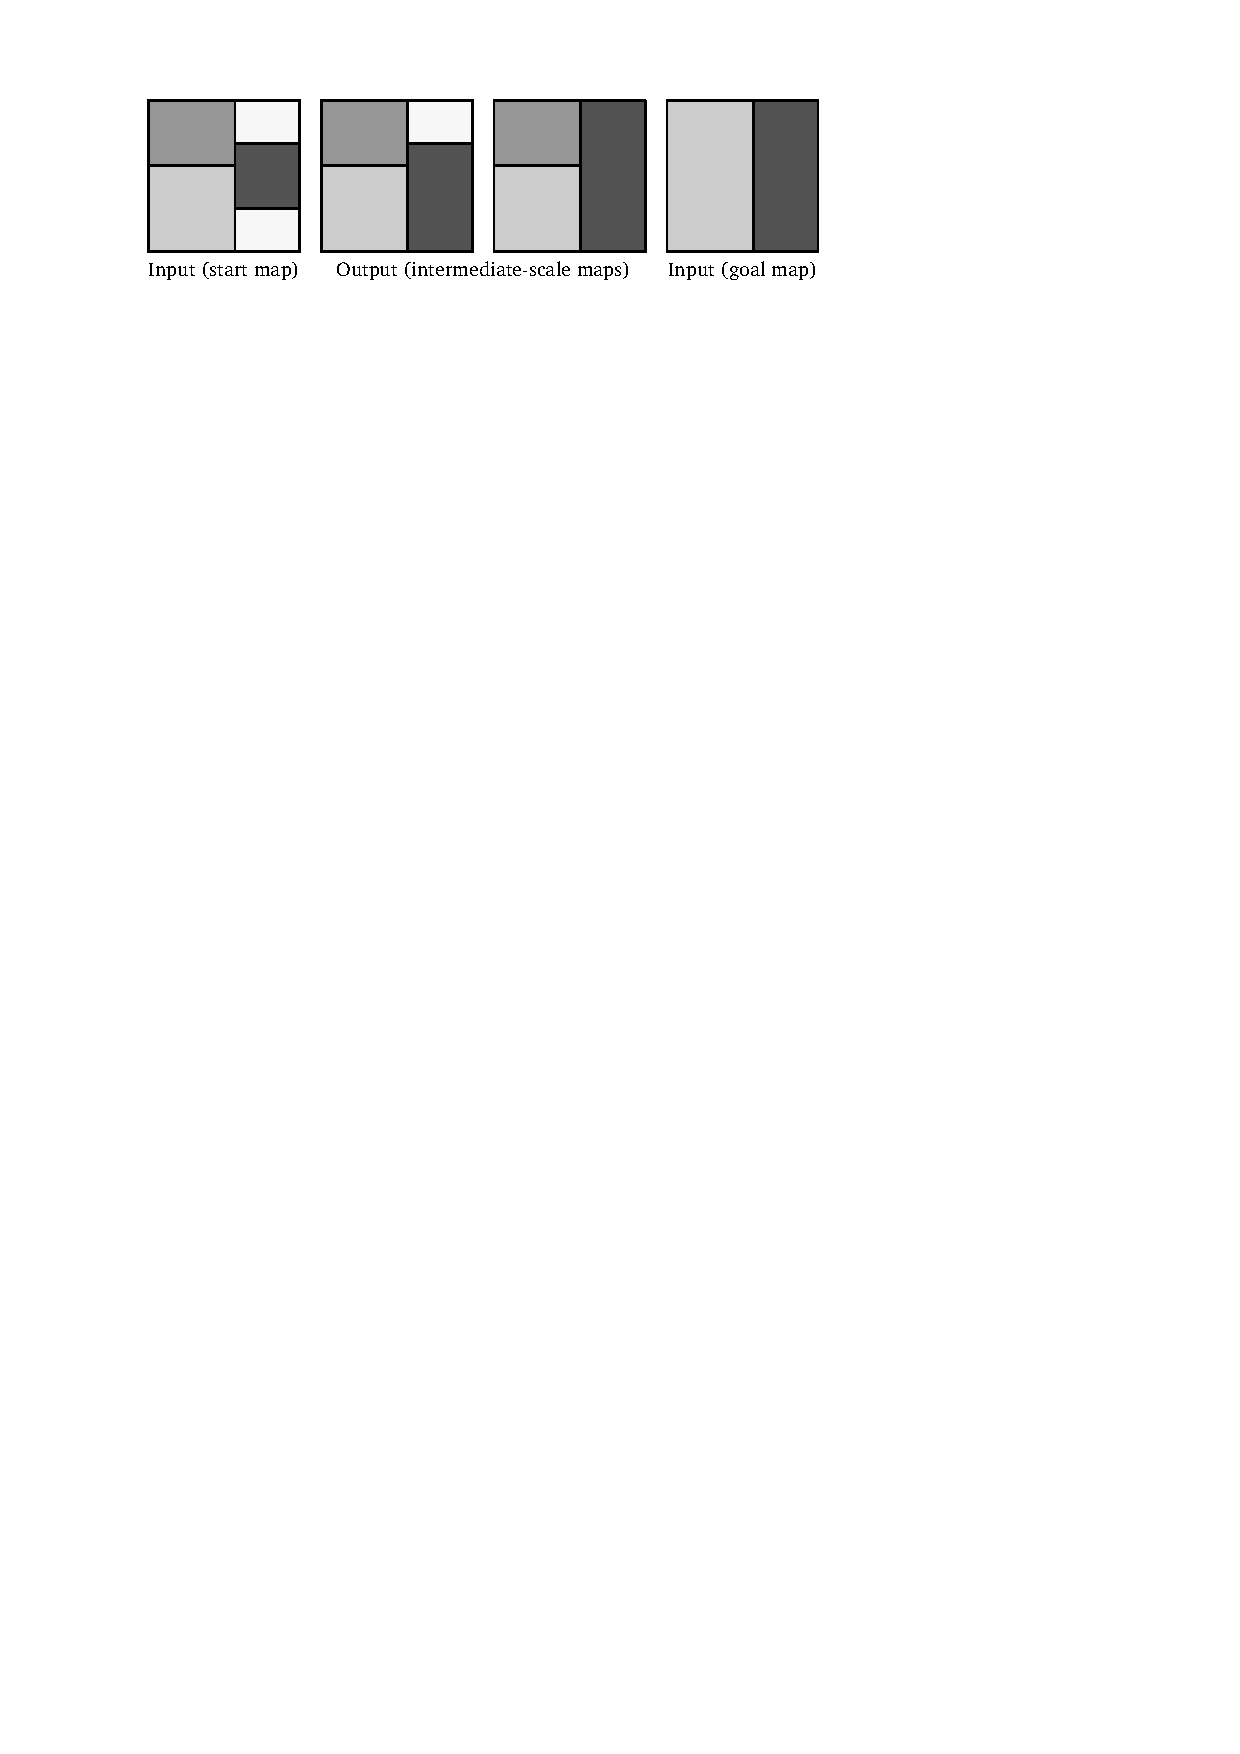
\includegraphics[page=1]{AreaAgg_Preliminaries}
	\caption{Integrating two aggregation sequences of different 
		regions: the resulting sequence contains the given 
		sequences as
		subsequences and always takes the subdivision with 
		smallest
		patch next}
	\label{fig:AreaAgg_IntegrateSequence}
\end{figure*}


To find a sequence of small changes that transforms the start 
map into the goal map,
we require that every change involves only two areas of the 
current map.
More precisely, in each step the smallest area $a$ is merged 
with one of its neighbors (adjacent areas) $b$
such that~$a$ and~$b$ are replaced by their union.
The union must take over the type of either~$a$ or~$b$. 
If the union uses the type of~$a$, 
we say that area~$b$ is \emph{aggregated into} area~$a$, 
and vice versa. 
How to aggregate exactly is decided by 
optimizing a global cost function.
This requirement ensures that the 
size of the smallest area in the map increases in each step
and thus the sequence reflects a gradual reduction of the 
map's scale.
From another perspective, 
we consider the smallest area as the least important, 
instead of involving more rules for importance, 
to avoid making our problem too complicated. 
Even though the requirement reduces the number of possible 
solutions,
there is still enough room for optimization 
since we leave open with
which of its neighbors the smallest area is aggregated.
We term a sequence of changes that adheres to our requirement an
\emph{aggregation sequence}.



\mypar{Model}
We consider a directed graph $G$, 
which we call the \emph{subdivision graph} 
(see \fig\ref{fig:AreaAgg_SubdivisionName}). 
The node set $V$ of~$G$ contains a node for every
possible map (or \emph{subdivision}, including the start map, all
possible intermediate-scale maps, and the goal map).
The arc set~$E$ of~$G$ contains an arc $\Pnode P_{t+1,j}$ 
between any two maps $\Pnode, P_{t+1,j} \in V$ 
if $P_{t+1,j}$ can be reached from $\Pnode$ 
with a single aggregation operation,
involving the smallest area.
Then, any directed path in~$G$ from the start map to the goal map
defines a possible aggregation sequence.
Our idea is to compute an optimal aggregation sequence through 
computing a minimum-weight path from start to goal.
This idea obviously requires that the arc weights are 
set such that a minimum-weight start--goal
path does actually correspond to an aggregation sequence of 
maximum cartographic quality.  
Moreover, putting the idea to practice is far from trivial 
since the graph $G$ can be huge as we will argue below.
We compare a greedy algorithm, \Astar, and an ILP-based algorithm
in solving this problem.
Note that we only know subdivisions 
$\Pstart$ and $\Pgoal$ at the beginning. 


\begin{figure}[tb]
	\centering
	\includegraphics[page=2]{AreaAgg_Preliminaries}
	\caption{The subdivision graph~$G$. 
		The nodes of the graph are the subdivisions. 
		There is an arc	from subdivision~\Pnode 
		to subdivision~${P}_{t+1,j}$ 
		if ${P}_{t+1,j}$ is the result of 
		aggregating the smallest area~$p$ of~\Pnode with a 
		neighbor of~$p$.}
	\label{fig:AreaAgg_SubdivisionName}
\end{figure}

\mypar{Notation}
We represent each land-cover area by a polygon with a type.
We denote by $P$ the set of polygons on start map.
We use~$p$, $q$, $r$, or~$o$ to denote polygons.
A \emph{patch} is a set of polygons whose union is connected. 
The patch also has property type.
We use~$u$ or~$v$ to denote patches.
To slightly abuse the notations, we also say patch~$p$
provided that polygon~$p$ is the ``core'' of the patch.


Recall that there are~$n$ land-cover areas on the start	map. 
Hence, the desired aggregation sequence consists of~$n-1$ steps. 
There are $n$ subdivisions on a path 
from the start map to the goal map. 
We use $t \in {T}=\{1,2,\dots,n\}$ to denote 
the \emph{time} of the path. 
When $t=1$, the subdivision consists of $n$ patches, 
and there is only $1$ patch remaining when $t=n$.
The subdivision graph consists of layers~${L}_1,\dots,{L}_n$, 
where layer ${L}_t=\{{P}_{t,1},\dots,{P}_{t,n_t}\}$
contains every possible subdivision~\Pnode\ with 
$n-t+1$ patches (see \fig\ref{fig:AreaAgg_ExponentialSize}).

\begin{figure}[tb]
	\centering
	\includegraphics[page=3]{AreaAgg_Preliminaries}
	\caption{An example to show that the size of our problem 
	has an exponential lower bound.}
	\label{fig:AreaAgg_ExponentialSize}
\end{figure}

\mypar{Exponential lower bound}
We now analyze the size of the subdivision graph~$G$.
% Consider an instance that consists of a start 
% map~${P}_{1,1}$
% with $n=2k$ unit squares in a row and a goal 
% map~${P}_{n,1}$
% that is simply the union of the $n$ squares, that is, an
% $(n\times1)$-rectangle.  One of the intermediate subdivisions in
% layer~${L}_{k+1}$---let's call 
% it~${P}_{k+1,1}$---consists of a row
% of~$k$ $(2\times1)$-rectangles.  A lower bound for the number of 
% nodes
% of~$G$ is the number of ways the $(2\times1)$-rectangles
% in~${P}_{k+1,1}$ can be subdivided into unit squares: 
% each way
% corresponds to a unique node in a layer between the start map
% and~${P}_{k+1,1}$.  Clearly, there are exactly 
% $2^k=2^{n/2}$
% ways.
%
% \mypar{Formalizing Area Aggregation as a Pathfinding Problem}
% We model our aggregation problem as 
% finding a shortest-path in the subdivision graph~$G$, which is 
% weighted.
% We define the weight of an edge
% as the cost of the corresponding aggregation step.
% We try to find a shortest path 
% from subdivision $\Pstart$ (the start map) to~\Pgoal (the goal 
% map) 
% using the \Astar algorithm or the ILP-based algorithm. 
% Once we have found a shortest path, 
% we can generate an optimal aggregation sequence.
% Note that we only know subdivisions 
% $\Pstart$ and $\Pgoal$ at the beginning. 
%
Consider an instance that consists of 
a start map with $n=2k+1$ rectangles in a row and
a goal map that is simply the union of the $n$ squares
(see \fig\ref{fig:AreaAgg_ExponentialSize}).
At layer~$L_{k+1}$, we need to remove~$k$ of the~$2k$ intermediate sticks. 
The number of our choices is ${{2k}\choose{k}} \ge 2^k = 2^{(n-1)/2}$.
As a result, the size of our problem has an exponential lower bound.


\section{Cost Functions}
\label{sec:AreaAgg_CostFunctions}
We consider three aspects of cost. 
First, we wish to minimize the total type change, 
over all aggregation steps. 
Second, we hope to maximize the sum of average compactnesses,
over all intermediate subdivisions.
Third, we want to minimize the number of edges,
over all intermediate subdivisions.
We see the number of edges as another kind of compactness. 
The more edges a map has, the less compact the map is.

\subsection{Cost of type change}
We define the cost of type change as follows.
Suppose that we are at the step of 
aggregating from subdivision $P_{s,i}$ to subdivision 
$P_{s+1,j}$. 
In this step, patch~$u$ is aggregated into patch~$v$
(see \figs\ref{fig:AreaAgg_FirstStep}a 
and \ref{fig:AreaAgg_FirstStep}b).
We denote the types of the two patches by~$T(u)$ and~$T(v)$. 
We define the cost of type change of this step by
\begin{equation}
\label{eq:f_type}
f_\mathrm{type}(P_{s,i},P_{s+1,j})=\frac{A_{u}}{A_R}
\cdot
\frac{d(T(u),T(v))}{T_{\max}},
\end{equation}
where variable~$A_u$ is the area of patch~$u$, 
and~$A_R$ is the area of region~$R$.
The constant~$T_{\max}$, the maximum cost over all type changes, 
is used to unify the cost of type change 
and is known from the input. 
The input specifies, for each pair~$(T_1,T_2)$ of types, 
the cost~$d(T_1,T_2)$ of changing type~$T_1$ to type~$T_2$.
Specifically, we denote by~$T_\mathrm{goal}$ the type of 
the only patch on goal map.


For path $\Pistar=(P_{1,i_1}, P_{2,i_2}, \dots, 
P_{\tstar,i_{\tstar}})$,
we define the cost of type change over the steps so far by
\begin{equation}
\label{eq:g_type}
g_\mathrm{type}(\Pistar)=
\sum_{s=1}^{t-1}f_\mathrm{type}(P_{s,i_s},P_{s+1,i_{s+1}})
\end{equation}

\begin{figure}[tb]
	\centering
	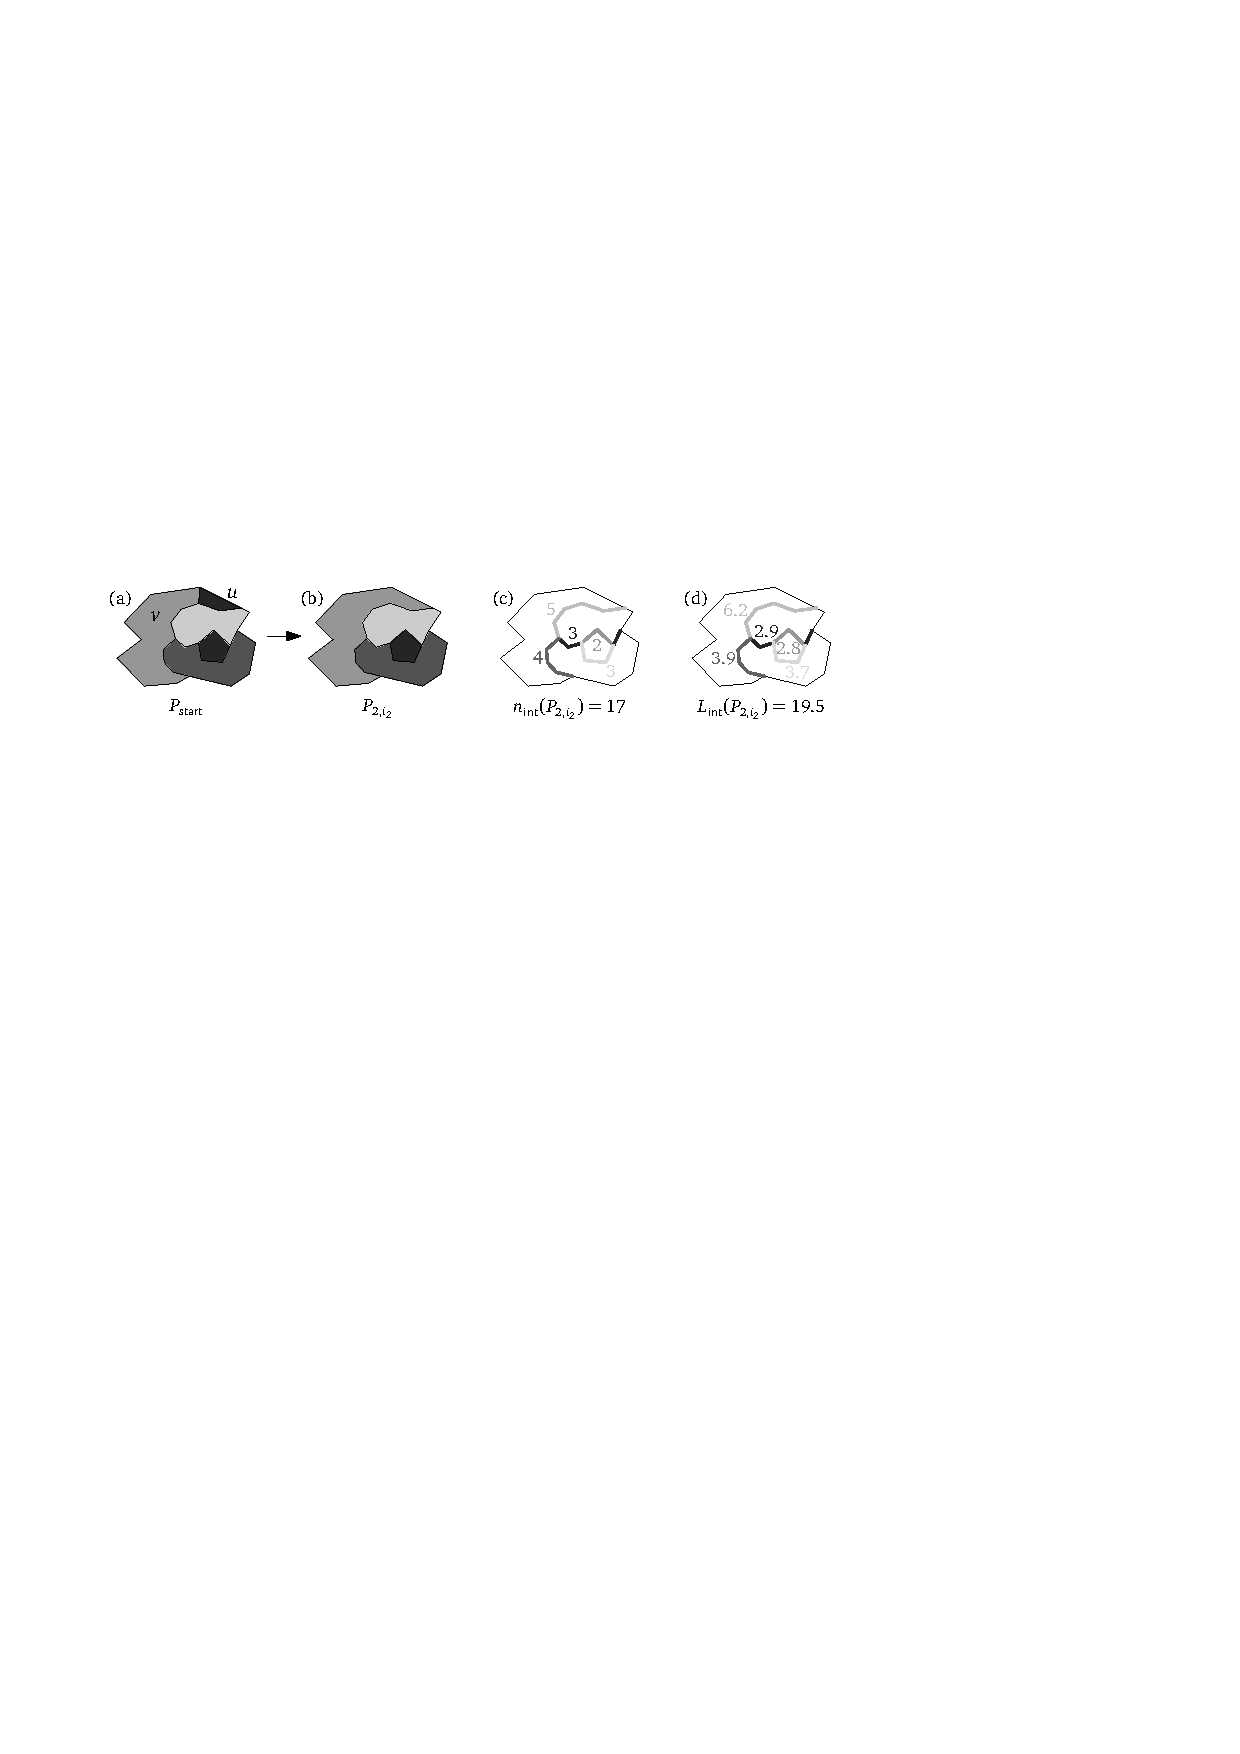
\includegraphics{AreaAgg_FirstStep}
	\caption{An aggregation step, 
	where patch~$u$, the dark patch at the top,
	is aggregated into patch~$v$, the gray patch to the left of~$u$.
	Figures~(c) and~(d) respectively show the number of edges and the lengths of the interior polylines.}
	\label{fig:AreaAgg_FirstStep}	
\end{figure}


%\begin{figure}[tb]
%	\begin{minipage}[b]{0.46 \linewidth}
%		\centering
%		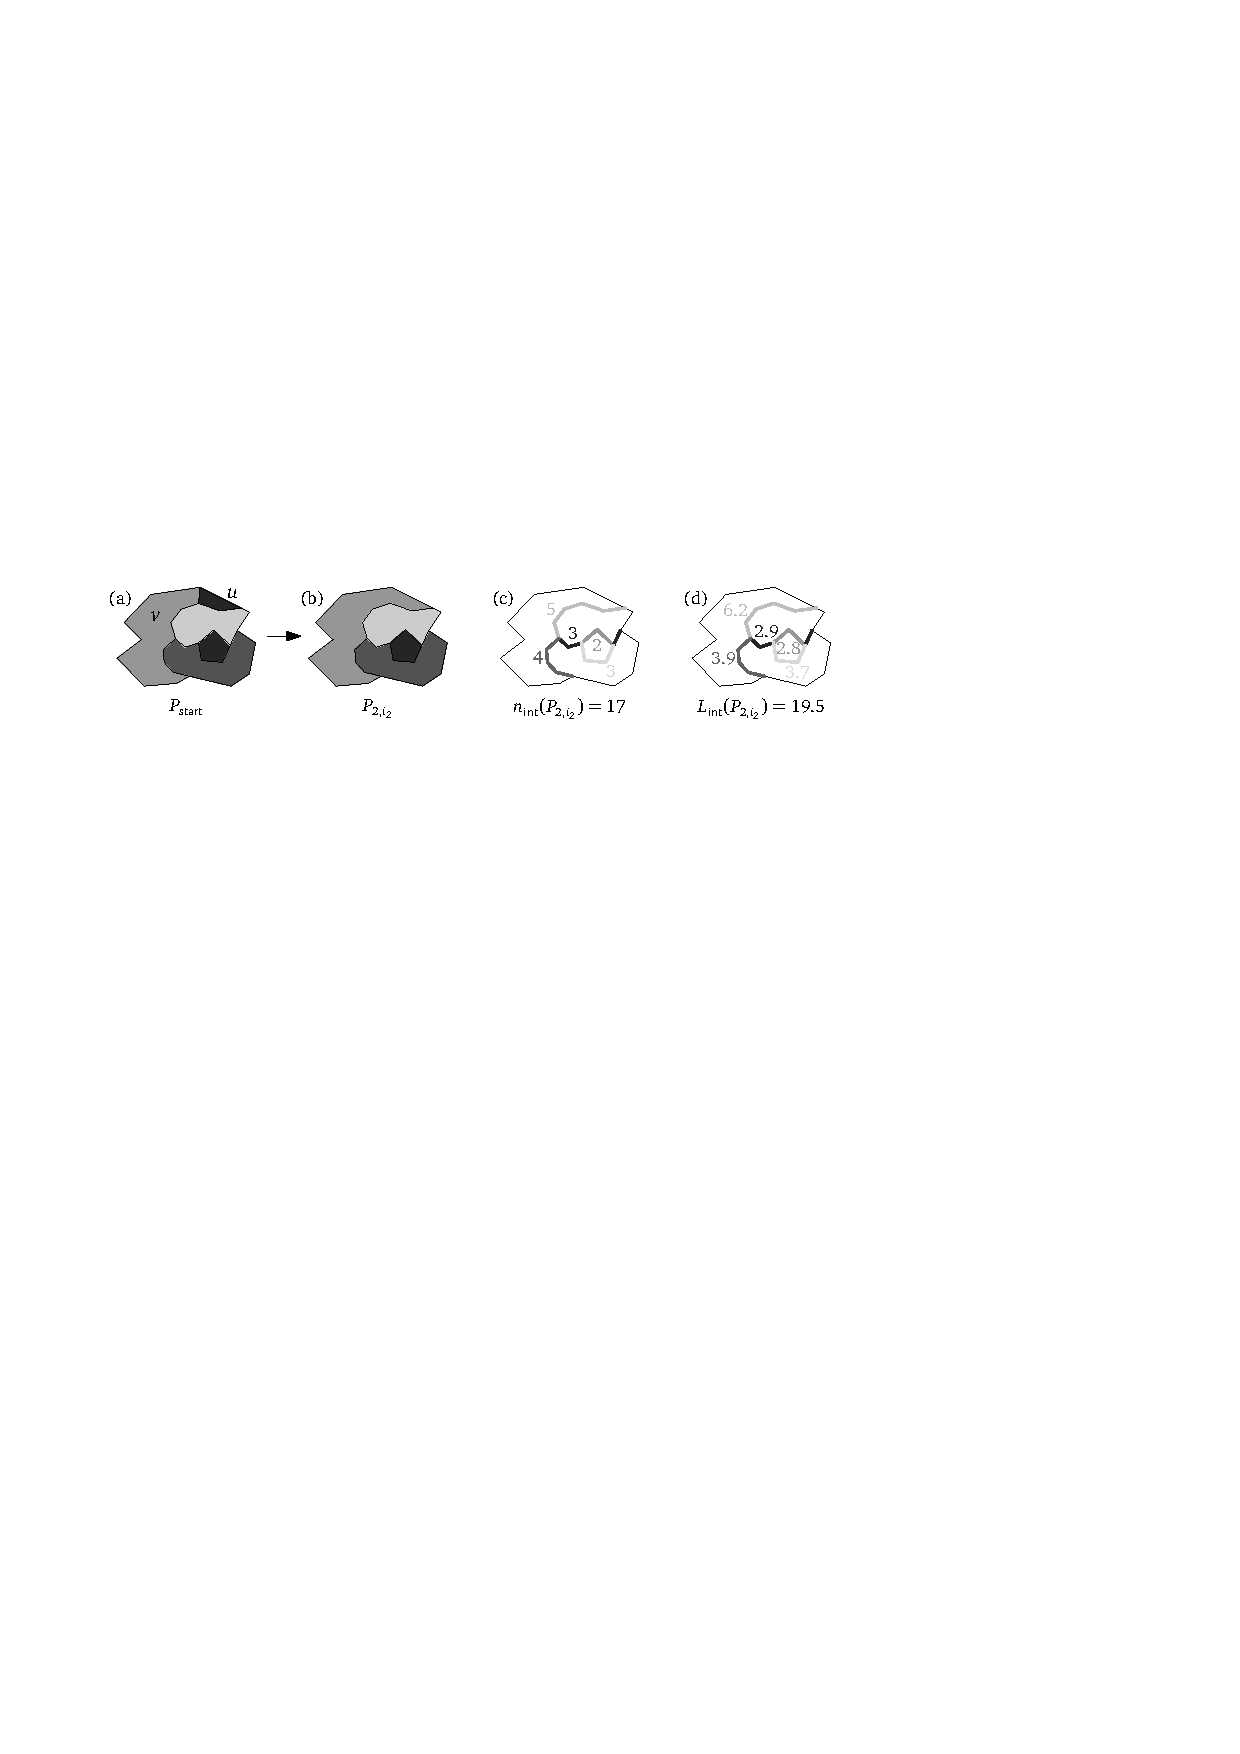
\includegraphics{AreaAgg_FirstStep}
%		\caption{An aggregation step, where the 
%			brown patch is aggregated into the green
%			patch.}
%		\label{fig:AreaAgg_FirstStep}
%	\end{minipage}
%	\hfil
%	\begin{minipage}[b]{0.48 \linewidth}
%		\centering
%		\includegraphics{AreaAgg_FirstStep_Costs}
%		\caption{The shaded parts show the contributions to the
%			costs.}
%		\label{fig:AreaAgg_FirstStep_Costs}
%	\end{minipage}	
%\end{figure}


\subsection{Cost of compactness}


We wish to maximize the sum of average compactnesses 
over all intermediate maps,
while our objective will be to minimize a cost.
To adapt the average compactness to our methods, 
we define and minimize a cost related to compactness, that is,
\begin{equation}
\label{eq:f_comp}
f_{\mathrm{comp}}(\Psnode)=
\frac{1-\frac{1}{n-s+1} \sum_{u\in \Psnode}c(u)}{n-2},
\end{equation}
where
\begin{equation}
\label{eq:comp}
c(u)=\frac{2 \sqrt{\pi A_u}}{l_u}
\end{equation}
is the compactness of patch~$u$ \citep{Frolov1975}, 
and $l_u$ is the perimeter of~$u$. 
We use~$n-2$ as the denominator to balance 
between the costs of type change and compactness.

For path $\Pistar$ (see \eq\ref{eq:g_type}), 
we define the cost of compactness over all 
intermediate subdivisions by
\begin{equation}
\label{eq:g_comp}
g_\mathrm{comp}(\Pistar)=
\sum_{s=2}^{\tstar-1}f_{\mathrm{comp}}(P_{s,i_s}).
\end{equation}


\subsection{Cost of length}
\label{sec:AreaAgg_costlength}

We want to make a comparison involving an ILP.
In an ILP, a linear cost function must be used.
As a matter of fact, most compactness measures, 
including $c_u$ in \eq\ref{eq:f_comp}, 
cannot be computed linearly
\parencite[see more measures in][]{Maceachren1985}.
We use the length of interior boundaries as a compactness index.
Although the length is not sufficiently precise 
to describe compactness 
\parencite[see for example][]{Young1988}, 
it is often used when compactness is considered in an ILP
\parencite[e.g.,][]{Minas2016,HaunertWolff2010AreaAgg,Wright1983}.
We denote the set of interior boundaries for a subdivision
$\Psnode$ by $B(\Psnode)$.
The cost in terms of interior length is defined as
\begin{equation}
\label{eq:f_length}
f_{\mathrm{length}}(\Psnode)=
\frac{\big(\sum_{b\in B (\Psnode)} 
|b|\big)\big/D(s)}{n-2}, 
\end{equation} 
where 
\begin{equation}
\label{eq:AreaAgg_Norm}
D(s)=\frac{n-s}{n-1} \sum_{b\in B (\Pstart)} |b|
\end{equation}
is the expected length of the interior boundaries at time~$s$. 
We use~$D(s)$ to somewhat normalize the cost of length. 
Similar to \eq\ref{eq:f_comp}, 
we use the value~$n-2$ 
to balance between the costs of type change and length.

For path~$\Pistar$ (see \eq\ref{eq:g_type}), 
we define the cost of length over all 
intermediate subdivisions by
\begin{equation}
\label{eq:g_length}
g_\mathrm{length}(\Pistar)=
\sum_{s=2}^{\tstar-1}f_{\mathrm{length}}(P_{s,i_s}).
\end{equation}



\subsection{Combining cost functions}
\label{sec:AreaAgg_Combining}
We define two combinations of cost functions.
The first combination is
\begin{equation}
\label{eq:g_1}
g_1(\Pistar)= (1-\lambda)g_\mathrm{type}(\Pistar)
+\lambda g_\mathrm{comp}(\Pistar),
\end{equation}
where $\lambda \in [0,1]$ is a parameter to balance 
between~$f_\mathrm{type}$ and~$f_\mathrm{comp}$.
In most cases, we use~$\lambda=0.5$ in our experiments. 
We want to find a path~$\Pi$ from~$\Pstart$ to~$\Pnode$ 
that minimizes, among all such paths,~$g(\Pistar)$.
Slightly abusing notation, we denote the length of
this shortest path from~${P}_{\mathrm{start}}$ to~\Pnode by~$g_1(\Pnode)$.
Using $g_1(\Pnode)$, we compare a greedy algorithm and \Astar
in finding optimal sequences for area aggregation.

The second combination is 
\begin{equation}
\label{eq:g_2}
g_2(\Pistar)= (1-\lambda)g_\mathrm{type}(\Pistar)
+\lambda g_\mathrm{length}(\Pistar).
\end{equation}
We compare a greedy algorithm, \Astar, and an ILP-based algorithm
using $g_2(\Pnode)$.



\section{A Greedy Algorithm}
\label{sec:AreaAgg_Greedy}
At any time $t$,
our greedy algorithm aggregates the smallest patch
with one of its neighbors.
Suppose that patch~$u$ is the smallest patch,
and patch~$v$ is one of~$u$'s neighbors.
We aggregate~$u$ into~$v$ 
if the type distances fulfill 
$d(T(u), T_\mathrm{goal})<d(T(v), T_\mathrm{goal})$.
Otherwise, we aggregate $v$ into $u$.
We compute the costs of aggregating the smallest patch 
with each of the neighbors, 
and select the aggregation that costs least.
In accordance 
with our two combinatorial costs in 
\sect\ref{sec:AreaAgg_Combining},
we define two cost functions.
Suppose that we are at the step of 
aggregating from subdivision $P_{s,i}$ to subdivision 
$P_{s+1,j}$.
The first cost function is 
\begin{equation}
\label{eq:f_1}
f_1(P_{s,i},P_{s+1,j})=
(1-\lambda)f_\mathrm{type}(P_{s,i},P_{s+1,j})
+\lambda f_{\mathrm{comp}}(P_{s+1,j}).
\end{equation}
The second cost function is
\begin{equation}
\label{eq:f_2}
f_2(P_{s,i},P_{s+1,j})=
(1-\lambda)f_\mathrm{type}(P_{s,i},P_{s+1,j})
+\lambda f_{\mathrm{length}}(P_{s+1,j}).
\end{equation}



\section{Using the \Astar Algorithm}
\label{sec:AreaAgg_AStar}


%\mypar[inline]{Motivate \Astar by comparison with Dijkstra.}


We try to find a shortest path,
from the start map to the goal map,
using \Astar \citep{Hart1968}.  
As the graph~$G$---our search space---can be of exponential size 
(see \sect\ref{sec:AreaAgg_Preliminaries}), 
we avoid computing the whole graph explicitly.
To save time and memory, 
we generate a subdivision \Pnode only 
when we are going to visit it.

\Astar uses a clever best-first search 
to find a shortest path 
from subdivisions~$\Pstart$ to~$\Pgoal$.  
For subdivision \Pnode,
\Astar considers the exact cost of a shortest path 
from~\Pstart to~\Pnode 
and estimates the cost to get from~\Pnode to~\Pgoal.  
\Astar can be seen as a refinement of Dijkstra's algorithm
where nodes are explored earlier 
if they are estimated to be closer to the goal.

More formally, we define $g(\Pnode)$ to be 
the exact cost of a shortest path from~\Pstart to~\Pnode, 
and we define $h(\Pnode)$ to be the estimated cost 
to get from \Pnode to~\Pgoal. 
Then the (estimated) total cost at node~\Pnode is
\begin{equation}
\label{eq:CostTotal}
F(\Pnode)=g(\Pnode)+h(\Pnode).
\end{equation}
If $h(\Pnode)$ is always bounded from above 
by the exact cost of a shortest path from~\Pnode to~\Pgoal, 
\Astar is guaranteed to find a shortest path from~\Pstart 
to~\Pgoal, 
that is, an optimal aggregation sequence.  
Using the estimation, \Astar is able to reduce the search space.
The better the estimation, the more \Astar can reduce the search 
space.
In the following, we show how we define $g(\Pnode)$ and 
$h(\Pnode)$.

To narrow down the search space, 
we set up estimation functions 
for type change (\sect\ref{sec:AreaAgg_h_type}), 
compactness (\sect\ref{sec:AreaAgg_h_comp}), 
and length (\sect\ref{sec:AreaAgg_h_length}). 
These functions are meant to direct \Astar towards the goal.

Since the number of subdivisions can be exponential, 
it happens that we run out of main memory 
before we find an optimal solution. 
To handle this problem, we overestimate the cost. 
Overestimation is a popular technique in \Astar,
in order to find a feasible solution. 
For example, \citet{Pohl1973} overestimated used dynamic 
weighting. 
We propose another strategy that fits our problem. 
We first try finding an optimal solution by \Astar. 
If we cannot find one after 
we have visited a predefined number~$M$ of nodes of graph~$G$,
then we restart the trying.
In the retrying, we overestimate $K$ steps for each node.
We may need to increase $K$ many times 
until we find a feasible solution.
We define $K$ by
\[
K= 2^k -1,
\]
where~$k\ge 0$ is the number of retryings.
As~$K \le n-1$, there holds~$k \le \log n +1$, 
which means  that we will 
retry~$\lceil \log n\rceil$ times at most.
When we are at time $t$, there are at most $n-t$ steps 
to arrive goal map.
We define the number of practical overestimation steps as
\[
K'= \min(K, n-t).
\]
Whenever overestimating ($k\geq1$), 
\Astar cannot guarantee optimality anymore.


\subsection{Estimating the cost of type change}
\label{sec:AreaAgg_h_type}

To find a lower bound of the cost of type change, 
we simply assume that 
every patch will be aggregated into a patch with type~\Tgoal.
As long as the cost of type change is a metric, this aggregation 
strategy indeed returns a lower bound.
%
For subdivision~\Pnode, let
$(P_{t,i_t}, P_{t+1,i_{\tstar+1}}, \dots,P_{n,i_n})$, 
$P_{t,i_t}=\Pnode$ and $P_{n,i_n}=\Pgoal$,
be the path that always changes the type of a smallest patch 
to~\Tgoal.
Then the estimated cost of type change is
\begin{equation}
	\label{eq:h_type}
	h_\mathrm{type}(\Pnode)=
\sum_{s=t}^{n-1}f_\mathrm{type}(P_{s,i_s},P_{s+1,i_{s+1}}).
\end{equation}

For an example, after the aggregation step of 
~\ref{fig:AreaAgg_FirstStep}, we compute $h_\mathrm{type}$ 
according to the aggregation sequence of 
\fig\ref{fig:AreaAgg_h_type}.
Note that the step from $P_{2,i_2}$ to 
$P_{3,i_3}$ 
in 
\fig\ref{fig:AreaAgg_h_type} is impossible in reality 
because the dark patch cannot be assigned patch~$v$
as they are not neighbors. 
However, this assignment is allowed for estimation 
because we may find a shortest path as long as 
the estimated cost is no more than 
the exact cost of a shortest path.
In order to overestimate, we time the estimated cost of the 
first $K'$ steps by $K$.
\fo\ref{eq:h_type} is revised to
\begin{equation}
\label{eq:o_type}
h_\mathrm{type}(\Pnode)=
K\sum_{s=t}^{t+K'-1}f_\mathrm{type}(P_{s,i_s},P_{s+1,i_{s+1}})+
\sum_{s=t+K'}^{n-1}f_\mathrm{type}(P_{s,i_s},P_{s+1,i_{s+1}}).
\end{equation}


\begin{figure*}[tb]
	\centering
	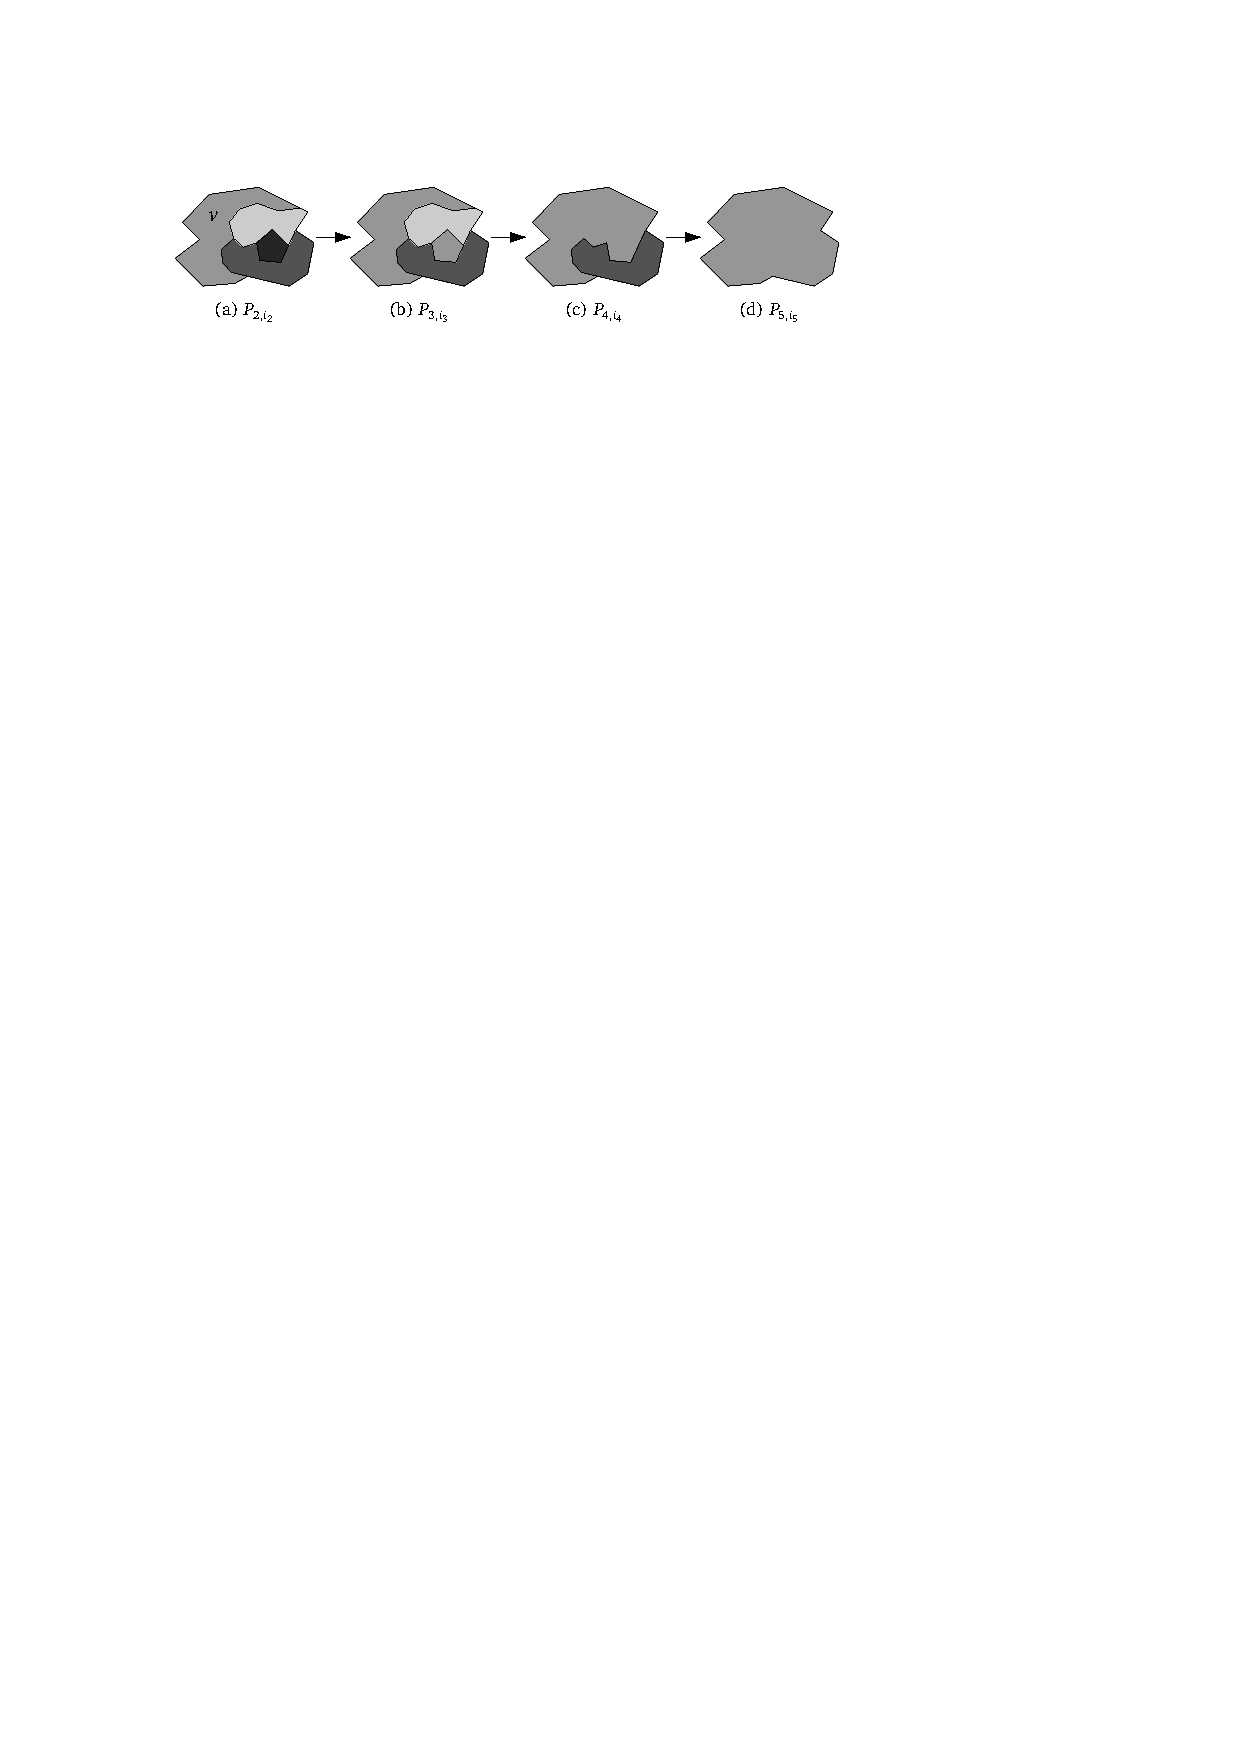
\includegraphics[page=1]{AreaAgg_Estimation}
	\caption{An ``aggregation sequence'' for computing 
		$h_{\mathrm{type}}$, 
		based on the aggregation result of 
		\fig\ref{fig:AreaAgg_FirstStep}b}
	\label{fig:AreaAgg_h_type}
\end{figure*}



%\mypar{Overestimation}





\subsection{Estimating the cost of compactness}
\label{sec:AreaAgg_h_comp}

Our way to estimate the cost of compactness 
is based on regular polygons.
The more edges a regular polygon has, the more compact it is.
We assume that at each step 
we aggregate the two patches that have the smallest 
compactnesses.
Moreover, the two patches happen to share the interior boundary 
which has the least number of edges.
We use $e_\mathrm{ext}$ to 
denote the edge number of the region's exterior boundaries.
As the exterior boundaries will not be changed by aggregation, 
$e_\mathrm{ext}$ 
is a constant. 
%
Note that a boundary between two patches is not necessarily 
connected 
(see for example the dark boundary with $3$ edges in
\fig\ref{fig:AreaAgg_h_comp}a).
We use $B(\Psnode)$ to denote the set of interior boundaries at 
time $s$,
and denote by $b_\mathrm{min}(\Psnode)$ 
the boundary having the smallest number of edges.
For our estimation, the set of interior boundaries at time $s+1$ 
is
$B(P_{s+1,j})= B(\Psnode)-{\{b_\mathrm{min}(\Psnode)\}}$. 
%
The number of interior edges at time $s+1$ is
\begin{equation}
\label{eq:LeftEdgeNum}
e_\mathrm{sum}(P_{s+1,j})=e_\mathrm{ext} + \sum_{b \in 
B(P_{s+1,j})} \|b\|.
\end{equation}
where $\|b\|$ is the number of edges of boundary~$b$.

\begin{figure*}[tb]
	\centering
	\includegraphics[page=2]{AreaAgg_Estimation}
	\captionof{figure}{An "aggregation" sequence for 
		computing 
		$h_\mathrm{comp}$ (see 
		\eq\ref{eq:o_comp}) based on the 
		number of edges. 
		At each step we remove the boundary with the fewest 
		edges. 		
		The numbers represent the 
		numbers of the interior boundaries' edges.
		This example corresponds to the aggregation step in 
		\fig\ref{fig:AreaAgg_FirstStep}.
	}
	\label{fig:AreaAgg_h_comp}
\end{figure*}


When we aggregate two patches, we have a new patch.
The compactness of this new patch is certainly smaller than 
a regular polygon with $e_\mathrm{sum}(P_{s+1,j})$ edges,
where a regular polygon with $e$ edges has compactness
\[
c_e=\sqrt{\frac{\pi}{e}\bigg/\tan{\frac{\pi}{e}}}
\]
Note that this expression increases with increasing $e$.
We denote by $c_\mathrm{reg} (P_{s+1,j})$ the compactness 
of the constructed regular polygon for subdivision 
$P_{s+1,j}$.
We use $C(\Psnode)$ to denote the set of compactnesses for 
subdivision $\Psnode$.
We denote the two smallest compactnesses by 
$c_\mathrm{min}(\Psnode)$ and $c'_\mathrm{min}(\Psnode)$.
Then the set of compactnesses for subdivision $P_{s+1,j}$ is 
\begin{equation}
\label{eq:compsetnew}
C(P_{s+1,j})=C(\Psnode) 
\cup \{c_\mathrm{reg} (P_{s+1,j})\} 
- \{c_\mathrm{min}(\Psnode), c'_\mathrm{min}(\Psnode)\}.
\end{equation}
Now we can compute the estimated average compactness by 
calculating the average 
of the elements in set $C(P_{s+1,j})$.

For subdivision~\Pnode, let
$(P_{t,i'_t}, P_{t+1,i'_{\tstar+1}}, \dots,P_{n,i'_n})$, 
$P_{t,i'_t}=\Pnode$ and $P_{n,i'_n}=\Pgoal$,
be the path that always removes the two smallest compactnesses
and gains a compactness of the constructed regular polygon.
The estimated cost of compactness is
\begin{equation}
\label{eq:h_comp}
h_\mathrm{comp}(\Pnode)=
\sum_{s=t}^{n-1}f_\mathrm{comp}(P_{s,i'_s}).
\end{equation}
When we overestimate, 
we assume that each patch is extremely noncompact,
that is, each patch has compactness~$0$.
The cost of compactness is $f_\mathrm{comp}(P_{s,i_s})=1/(n-2)$
according to \eq\ref{eq:f_comp}.
If we overestimate $K'$ steps, 
the estimated cost of compactness is revised to
\begin{equation}
\label{eq:o_comp}
h_\mathrm{comp}(\Pnode)=
\sum_{s=t}^{t+K'-1}\frac{1}{n-2}+
\sum_{s=t+K'}^{n-1}f_\mathrm{comp}(P_{s,i'_s}).
\end{equation}



\subsection{Estimating the cost of length}
\label{sec:AreaAgg_h_length}

At time $s$, there are $n-s+1$ patches.
There can be as few as $n-s$ interior boundaries.
In order to find a lower bound of the cost of length,
we at each step keep the necessary number ($n-s$) of shortest  
boundaries
(see \fig\ref{fig:AreaAgg_h_length}).
We compute the estimated cost of length according to 
\eq\ref{eq:f_length}.

For subdivision~\Pnode, let
$(P_{t,i''_t}, P_{t+1,i''_{\tstar+1}}, \dots,P_{n,i''_n})$, 
$P_{t,i''_t}=\Pnode$ and $P_{n,i''_n}=\Pgoal$,
be the path that always keeps 
the necessary number of shortest interior boundaries.
The estimated cost of length is
\begin{equation}
\label{eq:h_length}
h_\mathrm{length}(\Pnode)=
\sum_{s=t}^{n-1}f_\mathrm{length}(P_{s,i''_s}).
\end{equation}
When overestimating,
we use the interior length of the current map as the cost of 
length for $K'$ steps even though we are removing 
interior boundaries.
As a result, \fo\ref{eq:h_length} is revised to
\begin{equation}
\label{eq:o_length}
h_\mathrm{length}(\Pnode)=
\sum_{s=t}^{t+K'-1}f_\mathrm{length}(P_{t,i})+
\sum_{s=t+K'}^{n-1}f_\mathrm{length}(P_{s,i''_s}).
\end{equation}



%\begin{figure}[tb]
%	\centering
%	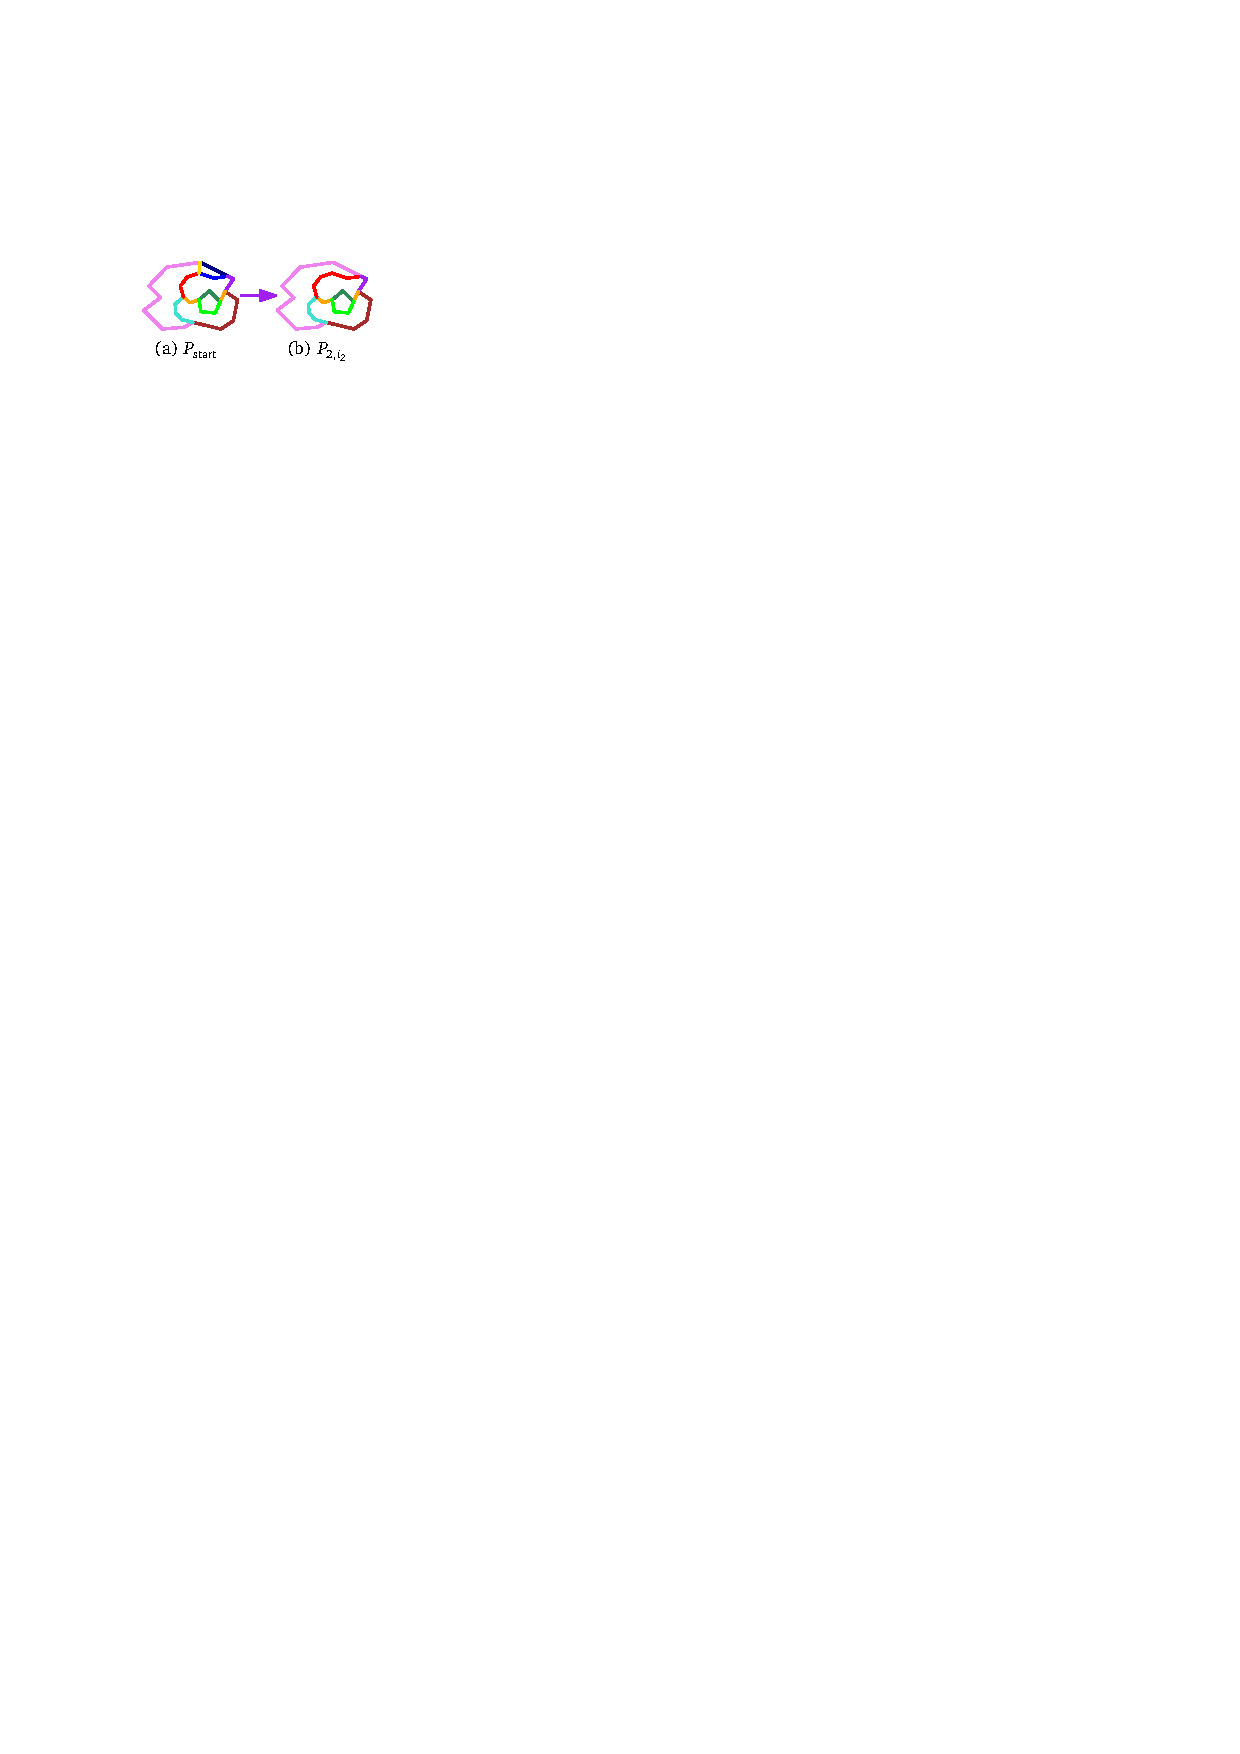
\includegraphics{AreaAgg_BoundaryChanging}
%	\caption{An example to show the change of the remained 
%		boundaries after removing a boundary. (a) Original 
%		boundaries. (b) The boundaries after the removing. This 
%		example 
%		corresponds to the aggregation step in 
%		\fig\ref{fig:FirstStep}. Note that the pink boundary 
%		and the navy boundary in (a) join together after we 
%		remove the yellow boundary, so do the 
%		red boundary and the blue boundary.}
%%	\label{fig:BoundaryChanging}
%\end{figure}



\begin{figure*}[htb]
	\centering
	\includegraphics[page=3]{AreaAgg_Estimation}
	\caption{An "aggregation" sequence for computing 
		$h_\mathrm{length}$ 
		(see Equation~\ref{eq:h_length}) 
		based on the length of boundaries. 
		At each step we remain the necessary number 
		of boundaries with least lengths in order to find a 
		lower bound of edge length of the interior boundaries 
		$l_\mathrm{int}(t)$. 
		The numbers represent the 
		lengths of the interior boundary boundaries.
		This example corresponds to the aggregation step in 
		\fig\ref{fig:AreaAgg_FirstStep}
	}
	\label{fig:AreaAgg_h_length}
\end{figure*}


\subsection{Combining estimated costs}
\label{sec:AreaAgg_CombinationEstimated}
In accordance 
with our two combinatorial costs in 
\sect\ref{sec:AreaAgg_Combining},
we define two estimated-cost functions.
The first one is 
\begin{equation}
\label{eq:h_1}
h_1(\Pnode)=
(1-\lambda)h_\mathrm{type}(\Pnode)
+\lambda h_{\mathrm{comp}}(\Pnode).
\end{equation}
The second estimated cost is
\begin{equation}
\label{eq:h_2}
h_2(\Pnode)=
(1-\lambda)h_\mathrm{type}(\Pnode)
+\lambda h_{\mathrm{length}}(\Pnode).
\end{equation}





\section{Integer Linear Programming}
\label{sec:AreaAgg_ILP}

Integer Linear programming is a method 
of finding optimal solutions for mathematical models.
In integer linear programming, 
the requirements and the objectives must be 
linear functions of the variables, 
and the variables must be integers; 
for more details, see 
\textcite[chapter~13]{Papadimitriou1982combinatorial}.
The general form of an integer linear program (ILP) is
\begin{align*} 
\mathrm{minimize} 	\quad	 & \bm{C}^\mathrm{T}\bm{X}  \\
\mathrm{subject~to} \quad	 & \bm{EX \le H}, \\
							 & \bm{X}\ge \bm{0}, \\
\mathrm{and} 		\quad	 & \bm{X} \in \mathbb{Z}^I,
\end{align*}
where~$C \in \mathbb{R}^I$, $H \in \mathbb{R}^J$,
and~$E$ is a $(J \times I)$-matrix over the reals.
The model means that 
we wish to minimize some cost subject to some constraints.
We want to compare the \Astar algorithm with 
the integer linear programming in finding 
optimal solutions for our aggregation problem. 
Since the integer linear programming
can handle only linear constraints, 
we define the compactness of a domain as 
the length of the domain's interior boundaries.

We define the \emph{center} of a patch as the polygon 
to which other polygons in the same patch are assigned. 
At the beginning, every patch consists of only one polygon, 
and this polygon is the center of the patch.
When we aggregate patch~$u$ into patch~$v$, 
all the polygons of~$u$ are assigned to the center of~$v$,
and the types of the polygons are changed to the type of the 
center.
Patch~$u$ disappears after being aggregated.
Note that all the polygons in a patch have the same type.
In the following, we show how to formalize our problem 
as an ILP.
For simplicity, we sometimes denote by \emph{patch~$r$} the 
patch using polygon~$r$ as the center at time~$t$.


\subsection{Variables}
\label{sub:variables}

Our problem is to decide 
which polygons are assigned to which centers.
Each question of the type 
``is polygon~$p$ assigned to center~$r$''
can be answered with ``yes'' or ``no''.
Hence, we use binary ($0$--$1$) variables in our ILP;
for more details, see \textcite[chapter~9]{bradley1977applied}.
We need five sets of variables.
%
The first set of variables is used to tell the program 
our rules for area aggregation.
We define 
$$
x_{t,p,r}\in \{0,1\} \qquad 
\forall t\in T, \forall p,r \in P 
$$
with $x_{t,p,r}=1$ if and only if 
polygon $p$ is assigned to polygon $r$ at time $t$. 
If a polygon is a center at time~$t$, 
then the polygon must be assigned to itself, 
that is, $x_{t,r,r}=1$
(see \fig\ref{fig:AreaAgg_Variables}).

\begin{figure*}[tb]
	\centering
	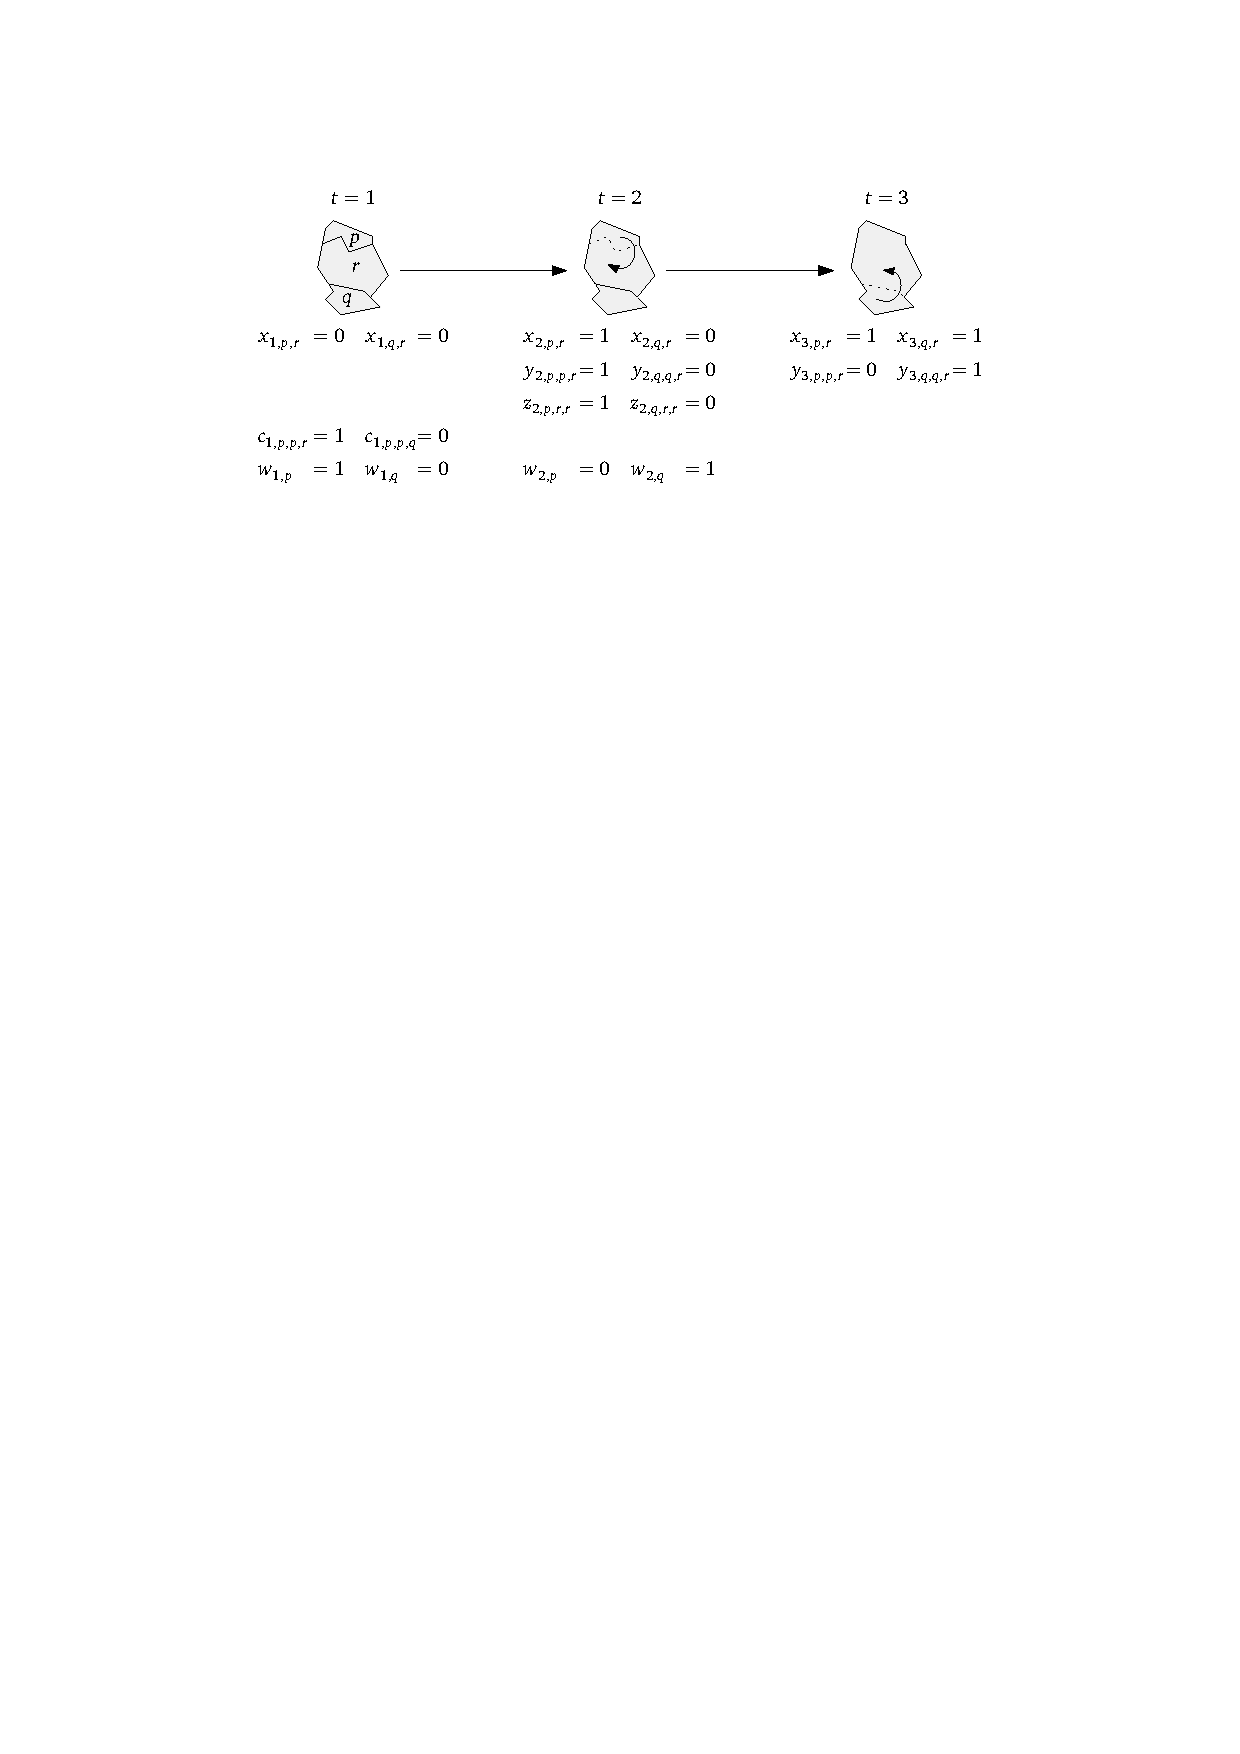
\includegraphics[page=1]{AreaAgg_ILP}
	\caption{Some examples of variables~$x_{t,p,r}$, 
		$y_{t,p,o,r}$, and~$z_{t,p,q,r}$. 
	}
	\label{fig:AreaAgg_Variables}
\end{figure*}


Our second set of variables is needed 
so that we are able to compute the cost of type.
We define 
$$
y_{t,p,o,r}\in \{0,1\} \qquad 
\forall t\in T\setminus \{1\}, \forall p,o,r \in P 
$$
with $y_{t,p,o,r}=1$ if and only if 
polygon~$p$ is assigned to center $o\in P$ at time~$t-1$ 
and to center~$r$ at time~$t$.
Specifically, $y_{t,p,o,o}=1$ means that
polygon~$p$ is assigned to the same center 
from~$t-1$ to~$t$ 
(see \fig\ref{fig:AreaAgg_Variables}).

We need our third set of variables 
for computing the cost of length.
We define 
$$
z_{t,p,q,r}\in \{0,1\} \qquad 
\forall t\in T\setminus \{1,n\}, \forall p,q,r \in P 
$$
with $z_{t,p,q,r}=1$ if and only if, at time~$t$,
polygons~$p$ and~$q$ are both in patch~$r$.
In this case, their common boundary should be removed
(see \fig\ref{fig:AreaAgg_Variables}).
When~$z_{t,p,q,r}=1$ and~$p=q$,
we define the length of their common boundary to be~$0$ 
because we shall not remove any.
We do not need~$z_{t,p,q,r}$ for time~$t=1$ 
because there are no two polygons in the same patch.
Namely, it always holds that~$z_{1,p,q,r}=0$, 
which does not help in our ILP.
We do not need~$z_{t,p,q,r}$ for time~$t=n$
because all the polygons are in the same patch.
It always holds that~$z_{n,p,q,r}=1$, 
which does not help in our ILP, either.

The fourth set of variables is used for 
guaranteeing contiguity inside patches. 
In other words, we aggregate two patches 
only when they are neighbors (close).
We define 
$$
c_{t,p,o,r}\in \{0,1\} \qquad 
\forall t\in T\setminus \{n-1,n\}, 
\forall p,o,r \in P \text{~with}~o\ne r,
$$
where $c_{t,p,o,r}=1$ if and only if at time~$t$
polygon~$p$ is assigned to center~$o$ 
and~$p$ has a neighbor assigned to center~$r$
(see \fig\ref{fig:AreaAgg_Variables_Neighbor}).
We do not need~$c_{t,p,o,r}$ for~$t=n-1$ 
because then, there are only two patches left 
and they must be neighbors.

\begin{figure}[tb]
	\centering
	\includegraphics[page=2]{AreaAgg_ILP}
	\caption{There are two patches, 
		which respectively use polygons~$o$ and~$r$ 
		as their centers.
		Polygons in the same patch 
		are separated by dotted lines.
		Polygon~$p$ is in patch~$o$ and~$p$ has two neighbors,
		polygons~$q_1$ and~$q_2$, assigned to center~$r$.
		In this case, patch~$o$ and patch~$r$ are neighbors 
		and can be aggregated. 
	}
	\label{fig:AreaAgg_Variables_Neighbor}
\end{figure} 

Our last set of variables is optional.  It can be used to enforce that 
we aggregate a smallest patch with a neighboring one at each step. 
We define 
$$
w_{t,o}\in \{0,1\} \qquad 
\forall t\in T\setminus\{n\}, \forall o \in P 
$$
with $w_{t,o}=1$ meaning 
that polygon~$o$ is the center of 
a smallest patch at time~$t$.
%and this patch is involved in the aggregation step 
%from~$t$ to~$t+1$.


\subsection{Objectives}
\label{sub:objectives}

Our aim is to minimize the weighted sum of the two costs, 
the cost of type change and the cost of length,
that is,
\begin{equation}
\label{eq:ilpcost}
\mathrm{minimize} \quad 
(1-\lambda)F_\mathrm{type} +\lambda F_\mathrm{length},
\nonumber
\end{equation}
where $\lambda$, as in \eq\ref{eq:g_1}, 
is a parameter to balance 
$F_\mathrm{type}$ and $F_\mathrm{length}$.

We want to minimize the overall cost of type changes of the 
polygons. 
We define the cost of these changes as
\begin{equation}
\label{eq:F_type}
F_\mathrm{type}=\sum_{t=2}^{n} \sum_{p\in P} \sum_{o\in P} 
\sum_{r\in P}
\bigg( \frac{a_p}{A_R} \cdot
\frac{d(T(o),T(r))}{T_{\max}}\cdot 
y_{t,p,o,r}\bigg),
\end{equation}
where, similar to \eq\ref{eq:f_type}, 
$a_p$ is the area of polygon~$p$,
$A_R$ is the area of the region, 
and~$T(o)$ and~$T(r)$ are the types of centers~$o$ and~$r$.
Note that~$y_{t,p,o,r}=1$ even if $o=r$
as long as polygon~$p$ is assigned to center~$o$ at time $t-1$
and assigned to center~$r$ at time~$t$.
In this case, $p$ is not necessarily involved in an aggregation 
step so there should be no cost concerning~$p$.
In our case, type distance~$d(T(o),T(r))=0$ if~$o=r$,
which ensures that there is no cost.
Therefore, $y_{t,p,o,r}=1$ is fine when $o=r$. 


We also want to minimize the overall interior lengths of all the 
intermediate maps.
As discussed in \sect\ref{sec:AreaAgg_costlength},
we need a cost that can be computed linearly.
We use the length of the interior boundaries 
as an alternative of compactness.
Recall that $B(\Pstart)$ is the set of interior boundaries 
at time $t=1$ (see \sect\ref{sec:AreaAgg_costlength}).
The sum of the normalized length of the remaining interior 
boundaries at all 
times can be 
computed as
\begin{equation}
\label{eq:F_length_raw}
F_\mathrm{length}
=\frac{1}{n-2} \sum_{t=2}^{n-1} 
\frac{\sum_{b\in B (\Pstart)} |b| - 
	\frac{1}{2} \sum_{p \in P}\sum_{q \in P}\sum_{r \in P} 
	\big(|b_{pq}|\cdot z_{t,p,q,r}\big)}
{D(t)},
\end{equation}
where $b_{pq}$ is the common boundary 
between polygons $p$ and $q$. 
We define $|b_{pq}|=0$ if $p=q$ 
because no boundary is removed in this case.
Function~$D(t)$, defined by \eq\ref{eq:AreaAgg_Norm}, 
is used to normalize the cost of length.
As the same as \eq\ref{eq:f_length}, 
$n-2$ is used to balance 
between the costs of type change and length.
Integrating~$D(t)$ into \eq\ref{eq:F_length_raw}, we have
\begin{equation}
\label{eq:F_length}
F_\mathrm{length}
=\frac{n-1}{n-2} \sum_{t=2}^{n-1}
\Bigg(
\frac{1}{n-t} -
\frac{\sum_{p \in P}\sum_{q \in P}\sum_{r \in P} 
	\big(|b_{pq}|\cdot z_{t,p,q,r}\big)}
{2(n-t)\sum_{b\in B (\Pstart)} |b| }
\Bigg).
\end{equation}




\subsection{Constraints}

In order to formulate our aggregation problem as an ILP, we use the
variables introduced in \sect\ref{sub:variables} to express 
constraints.
For the binary variables of type~$x_{t,p,r}$, recall that the intended
meaning of $x_{t,p,r}=1$ is that, at
time~$t$, polygon~$p$ is assigned to center~$r$. 
Our first constraint is that, at time~$t$, polygon~$p$ is assigned to 
exactly one center. To this end, we require 
that
\begin{equation}
\label{eq:CstrOneCenter}
\sum_{r\in P} x_{t,p,r}=1 \qquad
\forall t \in {T}, \forall p \in P.
\end{equation}

The next constraint is that polygon~$r$ must be a center
for other polygons to be assigned to~$r$.
In our problem, if~$r$ is a center, 
then it must be assigned to~$r$ itself,
that is, $x_{t,r,r}=1$.
If~$r$ is not a center, then $x_{t,r,r}=0$.
In either case,
\begin{equation}
\label{eq:CstrAssign}
x_{t,p,r} \leq x_{t,r,r} \qquad
\forall t \in {T}, \forall  p, r \in P.
\end{equation}

Aggregating one patch into another results in 
the number of centers decreasing by~$1$.
We make sure that exactly one patch 
is aggregated into another by 
specifying the number of centers
for each point in time, that is,
\begin{equation}
\label{eq:CstrCountCenter}
\sum_{r\in P} x_{t,r,r}=n-t+1 \qquad
\forall t \in {T},
\end{equation}
where polygon $r$ is a center at time~$t$ if and only if 
$x_{t,r,r}=1$.

A center can disappear, but will never reappear afterwards.
Hence,
\begin{equation}
\label{eq:CstrNoReappear}
x_{t,r,r} \geq x_{t+1,r,r} \qquad 
\forall t \in {T}\setminus \{n\},
\forall r \in P.
\end{equation}


On the start map, 
there are some polygons with  goal type $T_\mathrm{goal}$
(see definition in \sect\ref{sec:AreaAgg_h_type}).
At time $t=n$, all polygons are aggregated into one patch.
This patch must have the goal type $T_\mathrm{goal}$.
In other words, the center of this patch must be one of the 
polygons with the 
goal type on the start map:
\begin{equation}
\label{eq:CstrType}
\sum_{r\in P \colon T(r)=T_\mathrm{goal}} x_{n,r,r}=1,
\end{equation}
where $T(r)$ is the type of polygon $r$ at time $t=1$.

Next, we use the binary variables of type~$y_{t,p,o,r}$ that we
introduced in \sect\ref{sub:variables}.  Recall that the 
intended 
meaning of~$y_{t,p,o,r}=1$ is that polygon~$p$ is assigned to
center~$o$ at time $t-1$ and to center~$r$ at time~$t$.
To enforce this, we use two types of constraints.

First, if polygon~$p$ is assigned 
to center~$o$ at time~$t-1$ ($x_{t-1,p,o}=1$)
and assigned to center~$r$ at time $t$
($x_{t,p,r}=1$), then $y_{t,p,o,r}=1$.  This is expressed by
\begin{equation}
\label{eq:CstrY1}
y_{t,p,o,r}\geq x_{t-1,p,o}+x_{t,p,r}-1 \qquad
\forall t \in {T} \setminus \{1\}, 
\forall p, o, r \in P.
\end{equation}

Second, if~$p$ is not assigned to~$o$ at~$t-1$ ($x_{t-1,p,o}=0$)
or~$p$ is not assigned to~$r$ at time $t$ ($x_{t,p,o}=0$),
then $y_{t,p,o,r}=0$.
This is expressed by
\begin{equation}
\label{eq:CstrY2}
\begin{array}{l}
y_{t,p,o,r} \le x_{t-1,p,o} \\
y_{t,p,o,r} \le x_{t,p,r}
\end{array} 
\bigg\} \qquad 
\forall t\in T\setminus \{1\}, 
\forall	p,o,r \in P.	
\end{equation}

%Third, if centers $o$ and $r$ are identical, 
%then the center of polygon $p$ is not changed.
%In this case, $y_{t,p,o,r}=0$, which is presented by
%\begin{equation}
%\label{eq:CstrY3}
%y_{t,p,o,r}=0 \qquad
%\forall t \in {T} / \{n\}, 
%\forall p, o, r \in P.
%\end{equation}

In \sect\ref{sub:variables} we introduced binary variables of 
type~$z_{t,p,q,r}$.
Recall that the intended meaning of $z_{t,p,q,r}=1$ is that, at
time~$t$, polygons~$p$ and~$q$ are both in patch~$r$.
To enforce this, we need three types of constraints.

First, if two polygons~$p$ and~$q$ are assigned 
to center $r$ at time~$t$ ($x_{t,p,r}=x_{t,q,r}=1$),
then~$z_{t,p,q,r}=1$.  This is expressed by
\begin{equation}
\label{eq:CstrZ1}
z_{t,p,q,r}\geq x_{t,p,r}+x_{t,q,r}-1 \qquad
\forall t \in T \setminus \{1,n\}, 
\forall p, q, r \in P.
\end{equation}

Second, if $p$ or~$q$ is not assigned to~$r$,
then $z_{t,p,q,r}=0$.  This is expressed by
\begin{equation}
\label{eq:CstrZ2}
\begin{array}{l}
z_{t,p,q,r} \le x_{t,p,r} \\
z_{t,p,q,r} \le x_{t,q,r}
\end{array} 
\bigg\} \qquad 
\forall t\in T \setminus \{1,n\}, 
\forall	p,q,r \in P.	
\end{equation}

%Third, we introduce an abbreviation that will be helpful to 
%express
%the last type of constraint involving variables of 
%type~$z_{t,p,q,r}$:
%\begin{equation}
%\label{eq:CstrZabbrv}
%z_{t,p,q} = \sum_{r \in P}z_{t,p,q,r}
%\qquad 
%\forall t\in T \setminus \{1,n\}, 
%\forall	p,q \in P,
%\end{equation}
%where the reason we do not need~$z_{t,p,q}$ for~$t=1$ or~$t=n$
%is the same as for $z_{t,p,q,r}$
%(see \sect\ref{sub:variables}).
%Note that $z_{t,p,q}$ expresses whether, at time~$t$, 
%polygons~$p$ and~$q$ are 
%in the same patch ($z_{t,p,q}=1$) or not ($z_{t,p,q}=0$).
%%
%Note further that constraint~(\ref{eq:CstrZ2}) ensures that~$p$ 
%and~$q$
%can only be assigned to one common patch, that is, $z_{t,p,q} 
%\le 1$.

We use constraint~(\ref{eq:CstrTogether}) 
to express the following requirement. 
If two polygons have been aggregated into one patch, 
they will always be in the same patch 
at later times~-- although the center of their common patch 
can change after the point in time 
when they were aggregated first. 
In other words, as a function of~$t$, 
$z_{t,p,q}$ is monotonically increasing:
\begin{equation}
\label{eq:CstrTogether}
z_{t,p,q} \le z_{t+1,p,q} \qquad
\forall t \in \{2,3,\ldots,n-2\},  
\forall p, q \in P.
\end{equation}

The problem how to ensure contiguity inside a patch 
when using integer linear programming 
has received considerable attention.
Usually, a subdivision is represented by a graph
(see \fig\ref{fig:AreaAgg_Variables_Graph}).
%
\textcite{Zoltners1983Territory} regarded each node as a center.
For each center, they found a shortest path 
to each of the other nodes.
Then they required that a center can be assigned 
by a node only if 
at least one immediate predecessor of the node 
in the shortest path had been assigned to the center.
%
\textcite{Williams2002Contiguous} constructed a minimum spanning 
tree (MST) of the nodes.
They required that,
if some polygons are to be in the same patch,
the corresponding nodes must 
form a subtree of the MST.
%
Although this requirement makes their problem easier to be solved,
it excludes many feasible patches.
For a given center, \textcite{Cova2000_Contiguity} 
were able to find all the contiguous patches.
In their method, when a node is to be assigned to a center, 
a path from the node to the center was demanded 
that each node is assigned to the center.
%
Similarly, \textcite{Shirabe2005Contiguity} modeled 
the contiguity problem as a network flow.
He required that there must be a path so that 
some fluid could flow from a node to a sink (center).
%
These two ideas can be adapted into our method
as we do not wish to exclude any possible solutions.
However, we use another one,
which is more intuitive in terms of our problem
since we aggregate step by step.


\begin{figure}[tb]
	\centering
	\includegraphics[page=3]{AreaAgg_ILP}
	\caption{The graph of a subdivision.
		Each node of the graph represents a polygon in the 
		subdivision.
		There is an edge between two nodes
		if the corresponding two polygons are adjacent.
	}
	\label{fig:AreaAgg_Variables_Graph}
\end{figure} 

We want to aggregate two patches only if they are neighbors.
To ensure this, we need the binary variables of type $c_{t,p,o,r}$
that we introduced in \sect\ref{sub:variables}.
Recall that the intended meaning of $c_{t,p,o,r}=1$ is that, at time~$t$, 
polygon~$p$ of patch~$o$ has a neighbor polygon in patch~$r$.
To enforce this behavior of $c_{t,p,o,r}$, we need four types of
constraints.

First, at time~$t$, polygon~$p$ must be assigned to center~$o$,
\begin{equation}
\label{eq:CstrC_Part}
c_{t,p,o,r} \le x_{t,p,o} \qquad
\forall t 	 \in T\setminus \{n-1,n\},  
\forall p, o, r \in P \text{~with}~o\ne r.
\end{equation}

Second, at time~$t$, polygon~$p$ has at least 
one neighbor that is assigned to center~$r$,
\begin{equation}
\label{eq:CstrC_Neighbor}
c_{t,p,o,r} \le \sum_{q\in N(p)} x_{t,q,r} \qquad
\forall t 	 \in T\setminus \{n-1,n\},  
\forall p, o, r \in P \text{~with}~o\ne r.
\end{equation}

Third, if polygon~$p$ is in patch~$o$ and~$p$ has at least 
one neighbor in patch~$r$, then we must enforce~$c_{t,p,o,r}=1$,
\begin{equation}
\label{eq:CstrC_Positive}
c_{t,p,o,r} \ge x_{t,p,o} -1 +
\frac{\sum_{q\in N(p)} x_{t,q,r}}{n} \qquad
\forall t 	 \in T\setminus \{n-1,n\},  
\forall p, o, r \in P \text{~with}~o\ne r,
\end{equation}
where $N(p)$ represents the set of polygons adjacent to~$p$.
Recall that $n$ is the number of polygons on the goal map.
Polygon~$p$ can have~$n-1$ neighbors at most.
Hence, the last part of constraint~(\ref{eq:CstrC_Positive}),
$\left. \left(\sum_{q\in N(p)} x_{t,q,r}\right) 
\middle/ n \right.$,
is in the range~$[0,1)$.
As a result, if $x_{t,p,o}=1$ and the last part of 
constraint~(\ref{eq:CstrC_Positive}) is positive, 
then~$c_{t,p,o,r}$ must be~$1$.

Fourth, if we aggregate patch~$o$ into patch~$r$
between time steps~$t$ and $t+1$, 
then $y_{t+1,o,o,r}=1$.
In this case, we must make sure that 
the two patches are actually neighbors,
\begin{equation}
\label{eq:CstrC_Agg}
y_{t+1,o,o,r} \le \sum_{p\in P} c_{t,p,o,r} \qquad
\forall t 	 \in T\setminus \{n-1,n\},  
\forall o, r \in P \text{~with}~o\ne r.
\end{equation}


If we do not require that 
each aggregation step must involve a smallest patch,
then we only need constraints
(\ref{eq:CstrOneCenter})--(\ref{eq:CstrC_Agg})
explained so far 
and the variables of 
types~$x_{t,p,r}$, $y_{t,p,o,r}$, $z_{t,p,q,r}$,
and~$c_{t,p,o,r}$.
If we insist on involving a smallest patch at each step,
then we need more variables and more constraints.


\subsection{Aggregation involving a smallest patch}

We need another type of variable, ~$w_{t,o}$, 
in order to make sure that 
each of our aggregation steps involves a smallest patch.
We intend that~$w_{t,o}=1$ means 
that polygon~$o$ is the center of 
a smallest patch at time~$t$.
We will use this to enforce that
this patch is involved in the aggregation step 
from time~$t$ to~$t+1$.
At any time~$t$, there must be a smallest patch.
Therefore, we have
\begin{equation}
\label{eq:CstrSOneSmallest}
\sum_{o\in P}w_{t,o} =1 \qquad 
\forall t \in {T}\setminus \{n\}.
\end{equation}

Assume that patch~$o$ is the smallest patch
which is involved in the aggregation step from~$t$ to~$t+1$,
and that we are aggregating patches~$o$ and~$r$.
There can be two cases.
Patch~$o$ is aggregated into patch~$r$, or vice versa.
In the first case, we have~$y_{t+1,o,o,r}=1$,
and in the second case, we have~$y_{t+1,r,r,o}=1$.
Either of the two constraints implies 
that~$o$ is indeed a center at time~$t$, that is, $x_{t,o,o} =1$.
In order to enforce that
an aggregation step involves a smallest patch,
we must make sure that 
either $y_{t+1,o,o,r}=1$ or $y_{t+1,r,r,o}=1$ 
when $w_{t,o}=1$.
Consequently, we use constraint
\begin{equation}
\label{eq:CstrSInvolveSmallest}
w_{t,o} \le 
\sum_{r\in P\setminus \{o\}} y_{t+1,o,o,r} + 
\sum_{r\in P\setminus \{o\}} y_{t+1,r,r,o} \qquad
\forall t \in 
{T}\setminus \{n\}, \forall o \in P.
\end{equation}
We sum over all~$r\in P\setminus \{o\}$
so that this constraint is effective.
Otherwise, this constraint holds even if 
there is no smallest patch involved.

Now we need to make sure that 
the polygon~$o$ with $w_{t,o}=1$ is indeed 
the center of the smallest patch.
We define $A_{t,r}$ as the area of 
the patch using~$r$ as its center at time~$t$, 
that is,
\[
A_{t,r}=\sum_{p\in P} a_p \cdot x_{t,p,r},
\] 
where~$a_p$ is the area of polygon~$p$ 
and is a constant (as viewed by the ILP).
Area~$A_{t,r}$ is positive 
if and only if~$r$ is a center at time~$t$,
that is, if and only if~$x_{t,r,r}=1$.
We define a 
very large number~$W$ to help us construct constraints.
It suffices to set~$W$ to 
the area of the whole subdivision, i.e., \Pgoal. 
We require that
\begin{equation}
\label{eq:CstrSIndeedSmallest}
A_{t,o}-W(1-w_{t,o}) \le A_{t,r}+W(1-x_{t,r,r}) \qquad
\forall t 	 \in {T}\setminus \{n\}, 
\forall o, r \in P.
\end{equation}
This constraint only takes effect when $w_{t,o}=1$ and 
$x_{t,r,r}=1$, which indicates that 
the patch using polygon~$o$ as its center 
is smaller than or equal to all the other existing 
patches at time~$t$.

In order to compute an aggregation sequence 
involving a smallest patch at each step, 
we need all the five types of variables and 
constraints~(\ref{eq:CstrOneCenter})--(\ref{eq:CstrSIndeedSmallest}).


%\bigskip\bigskip\bigskip\bigskip\bigskip\bigskip\bigskip
%\bigskip\bigskip\bigskip\bigskip\bigskip\bigskip\bigskip

\section{Case Study}
\label{sec:AreaAgg_CaseStudy}
We have implemented our methods 
based on C\# (Microsoft Visual Studio 2015) 
and ArcObjects SDK 10.4.1.
We use IBM ILOG
CPLEX Optimization Studio 12.6.3.0 to solve our ILP. 
We ran our case study under~64-bit 
Windows~7 on a~$3.3\,$GHz dual core CPU with~$8\,$GB RAM.
We measured processing time 
by the built-in C\# class \emph{Stopwatch}.
As we run our program under a 32-bit platform, 
we added a post-build task about ``largeaddressaware''
in Microsoft Visual Studio
so that we were able to use up to 3 GB of main memory\footnote{
The details of the setting can be found at 	
\url{http://stackoverflow.com/questions/2597790/can-i-set-largeaddressaware-from-within-visual-studio},
Accessed: 2017-11-01.}.
Our CPLEX  version may declare an optimal solution
while it is not really optimal.
To fix this problem, we had to disable 
both primal and dual presolve reductions\footnote{
For more details about the problem, see
\url{http://www-01.ibm.com/support/docview.wss?uid=swg1RS02094},
Accessed: 2017-11-12.}.

We tested our method on a dataset 
from the German topographic database ATKIS DLM 50. 
The dataset represents the place 
``Buchholz in der Nordheide'' at scale $1:50{,}000$. 
Our start map is the map after the collapse of areas 
by \citet[pp.~61--66]{haunert2008f}, 
which has $5{,}537$ polygons. 
Our goal map was generalized from the start map 
by \citet{HaunertWolff2010AreaAgg} setting the scale 
at $1:250{,}000$ (see \fig\ref{fig:AreaAgg_Data}). 
The goal map has $734$ polygons, 
which means that there are $\mathcal{N}=734$ regions.  
%
We used a tree-based method introduced by \citet{Schwering2008} 
to define the cost of type change; 
the cost is the distance 
between two types in the type hierarchy\footnote{
More information about land-cover types can be found at 
\url{http://www.atkis.de/dstinfo/dstinfo2.dst_gliederung},
Accessed: 2017-11-01.}. 
(see \fig\ref{fig:AreaAgg_TypeDistances}). 
For example, the distance 
between type fence and type street is $4$.
In this tree, the maximum distance is $6$, 
which means $T_\mathrm{max}=6$ for \eq\ref{eq:f_type}.  

\begin{figure}[tb]
	\centering
	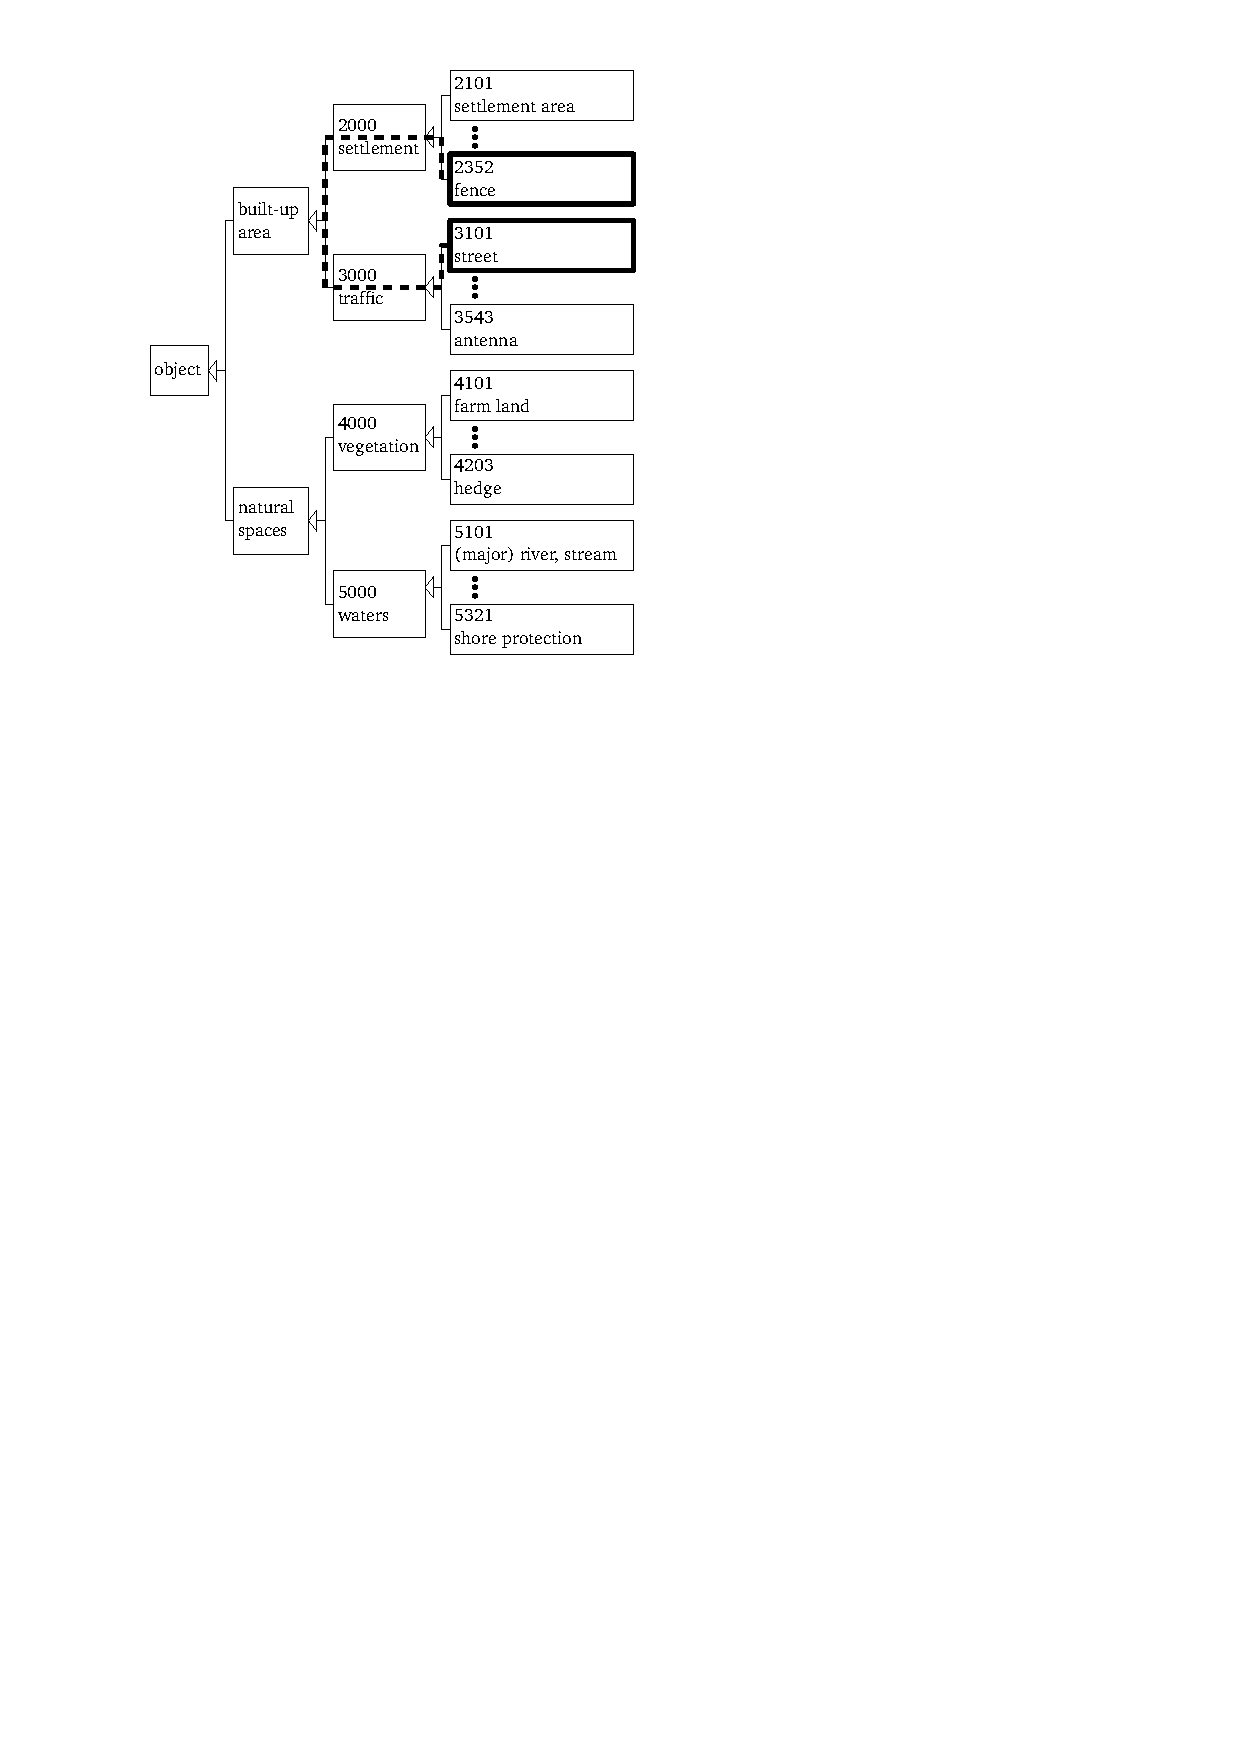
\includegraphics{AreaAgg_TypeDistances}
	\caption{The type distance defined in our case study. 
		For example, the distance 
		between type fence and type street is $4$.}
	\label{fig:AreaAgg_TypeDistances}
\end{figure}

\begin{figure}[tb]
	\captionsetup[subfigure]{labelformat=empty}
	\begin{subfigure}[b]{.49\textwidth}
		\centering
		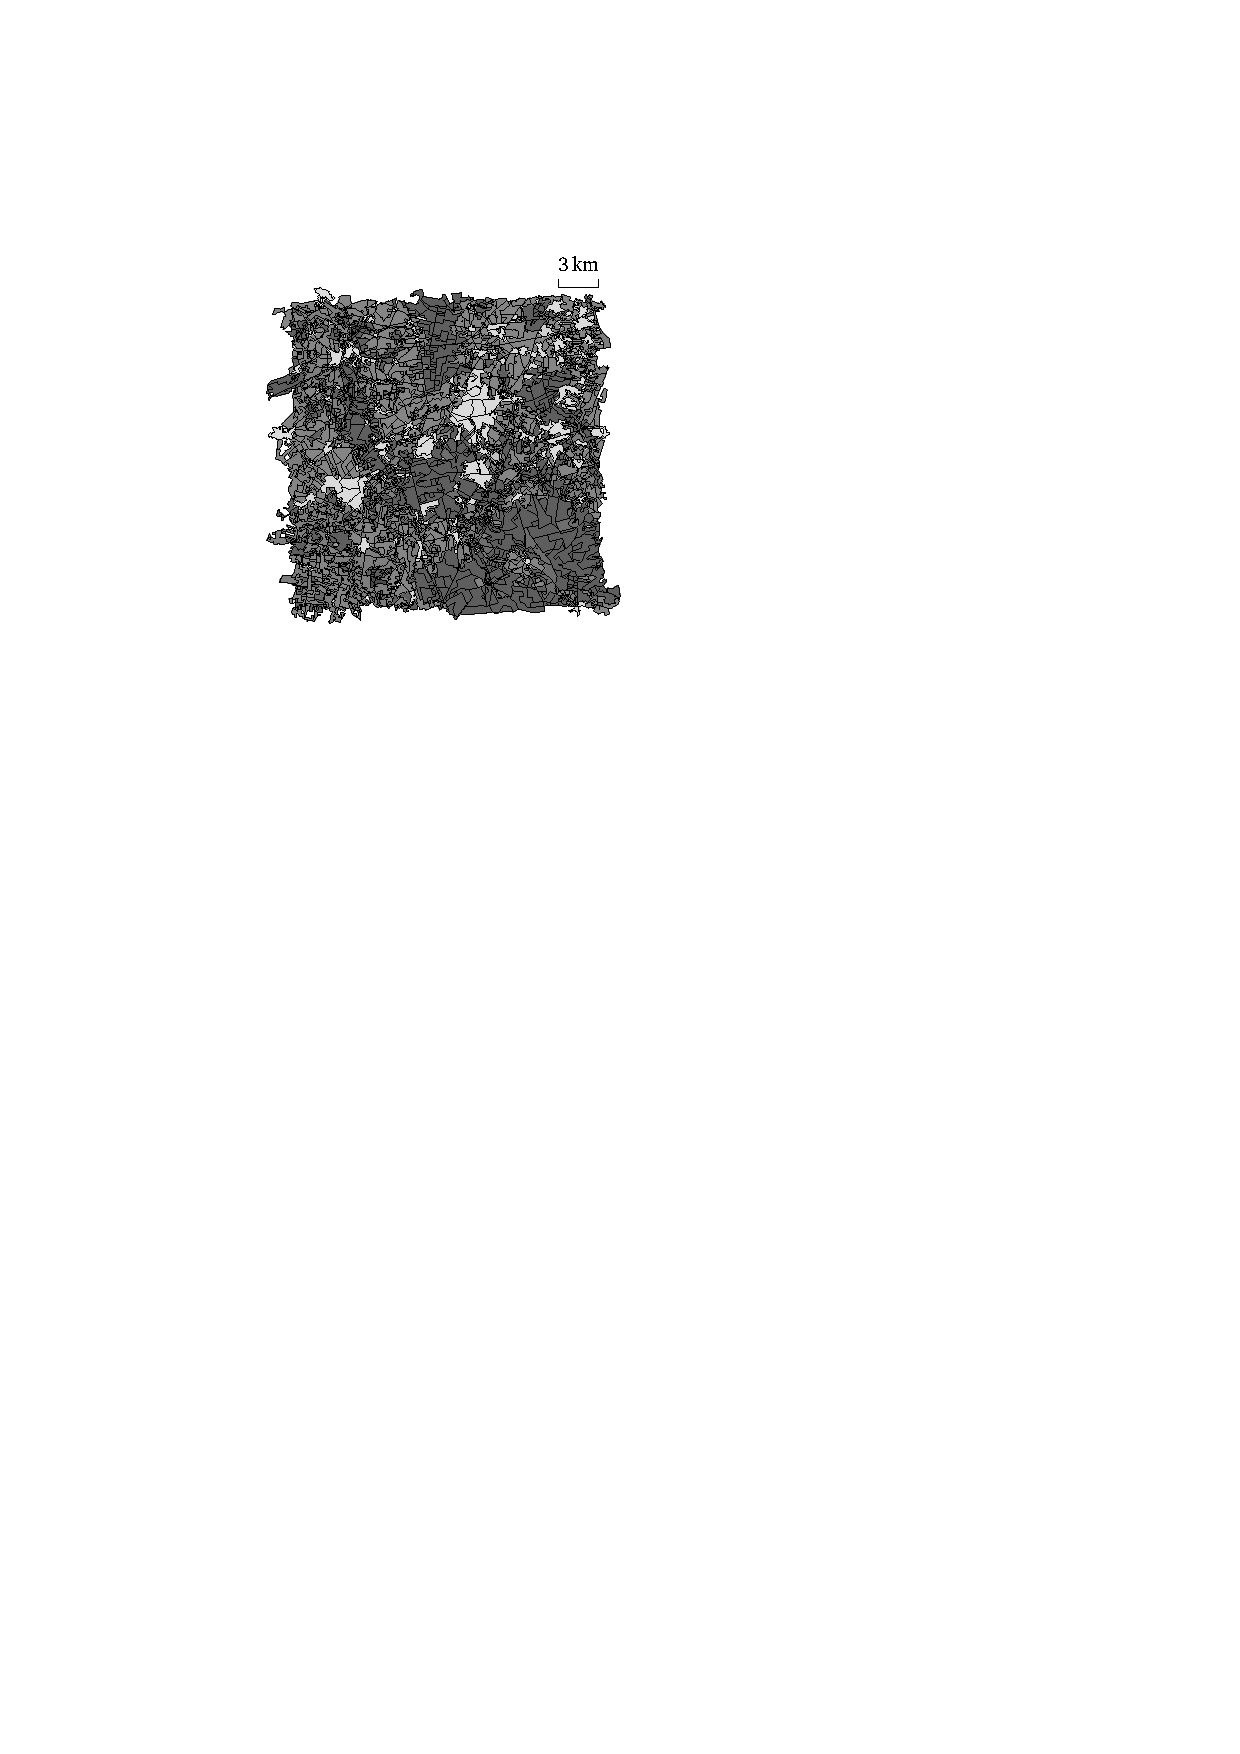
\includegraphics[page=1]{AreaAgg_Data}
		\caption{Start map, $5{,}537$ polygons, \\
			at scale $1:50{,}000$}
	\end{subfigure}
	\hfill
	\begin{subfigure}[b]{.49\textwidth}
		\centering
		\includegraphics[page=2]{AreaAgg_Data}
		\caption{Goal map, $734$ polygons, \\
			at scale $1:250{,}000$}
	\end{subfigure}
	
	\bigskip
	
	\begin{subfigure}{\textwidth}
		\centering
		\includegraphics[page=3]{AreaAgg_Data}
		\caption{The 20 land-cover types appearing in our data}
	\end{subfigure}
	\caption{The data of our case study.}
	\label{fig:AreaAgg_Data}
\end{figure}

\subsection{Using costs of type change and compactness}
As illustrated in \sect\ref{sec:AreaAgg_Combining},
we compare \Astar and our greedy algorithm using $g_1(\Pnode)$,
which is a combination of the costs 
of type change and compactness (see \eq\ref{eq:g_1}).

For \Astar, we overestimated 
whenever we could not find a solution after 
having visited~$M$ nodes (see 
Sec.~\ref{sec:AreaAgg_AStar}).
We tried $M=200{,}000$ and $M=400{,}000$. 
The results are shown in Table~\ref{tab:AreaAgg_CaseStudy1_Statistics}.
%
Unsurprisingly, the greedy algorithm visited fewer nodes and 
arcs in the graph $G$ than \Astar.
Using more running time, 
\Astar managed to reduce the cost 
from $120.7$ to $117.3$ (or $117.2$), 
which is $2.8\%$ less.
%
When $M=200{,}000$, 
we have found optimal aggregation sequences for 
$702$ of the $734$ regions, 
and found feasible sequences 
for the other $32$ regions ($94.3\%$); 
see column \#over in Table~\ref{tab:AreaAgg_CaseStudy1_Statistics}.
\begin{table*}[tb]
	%\small	
	\centering
	\caption{A comparison of Greedy and \Astar		
			when using cost function~$g_1$.
			For \Astar, we used two settings, 
			i.e.,~$M=200{,}000$ and~$M=400{,}000$.
		%
		Symbol~\#over is the number and percentage of regions
		(out of 734) that needed overestimation.
		%
		Variable~$k_\mathrm{sum}$ is the total repetitions.
		%
		Symbols~\#nodes and~\#arcs are the total 
		numbers of nodes and arcs that \Astar visited.  
		(For instances where we needed overestimation, 
		only the final attempt was counted.)
		%
		Symbols $g_\mathrm{t}$, $g_\mathrm{c}$, and $g_1$
		denote the sums of $g_\mathrm{type}(\Pgoal)$,
		$g_\mathrm{comp}(\Pgoal)$, and $g_1(\Pgoal)$,
		respectively, over all instances (see 
		\eqs\ref{eq:g_type}, \ref{eq:g_comp}, 
		and~\ref{eq:g_1}).
		%
		The percentage in the
		time column is the fraction of the total
		runtime spent on solving the instances
		that needed overestimation.
	}
	\label{tab:AreaAgg_CaseStudy1_Statistics}
	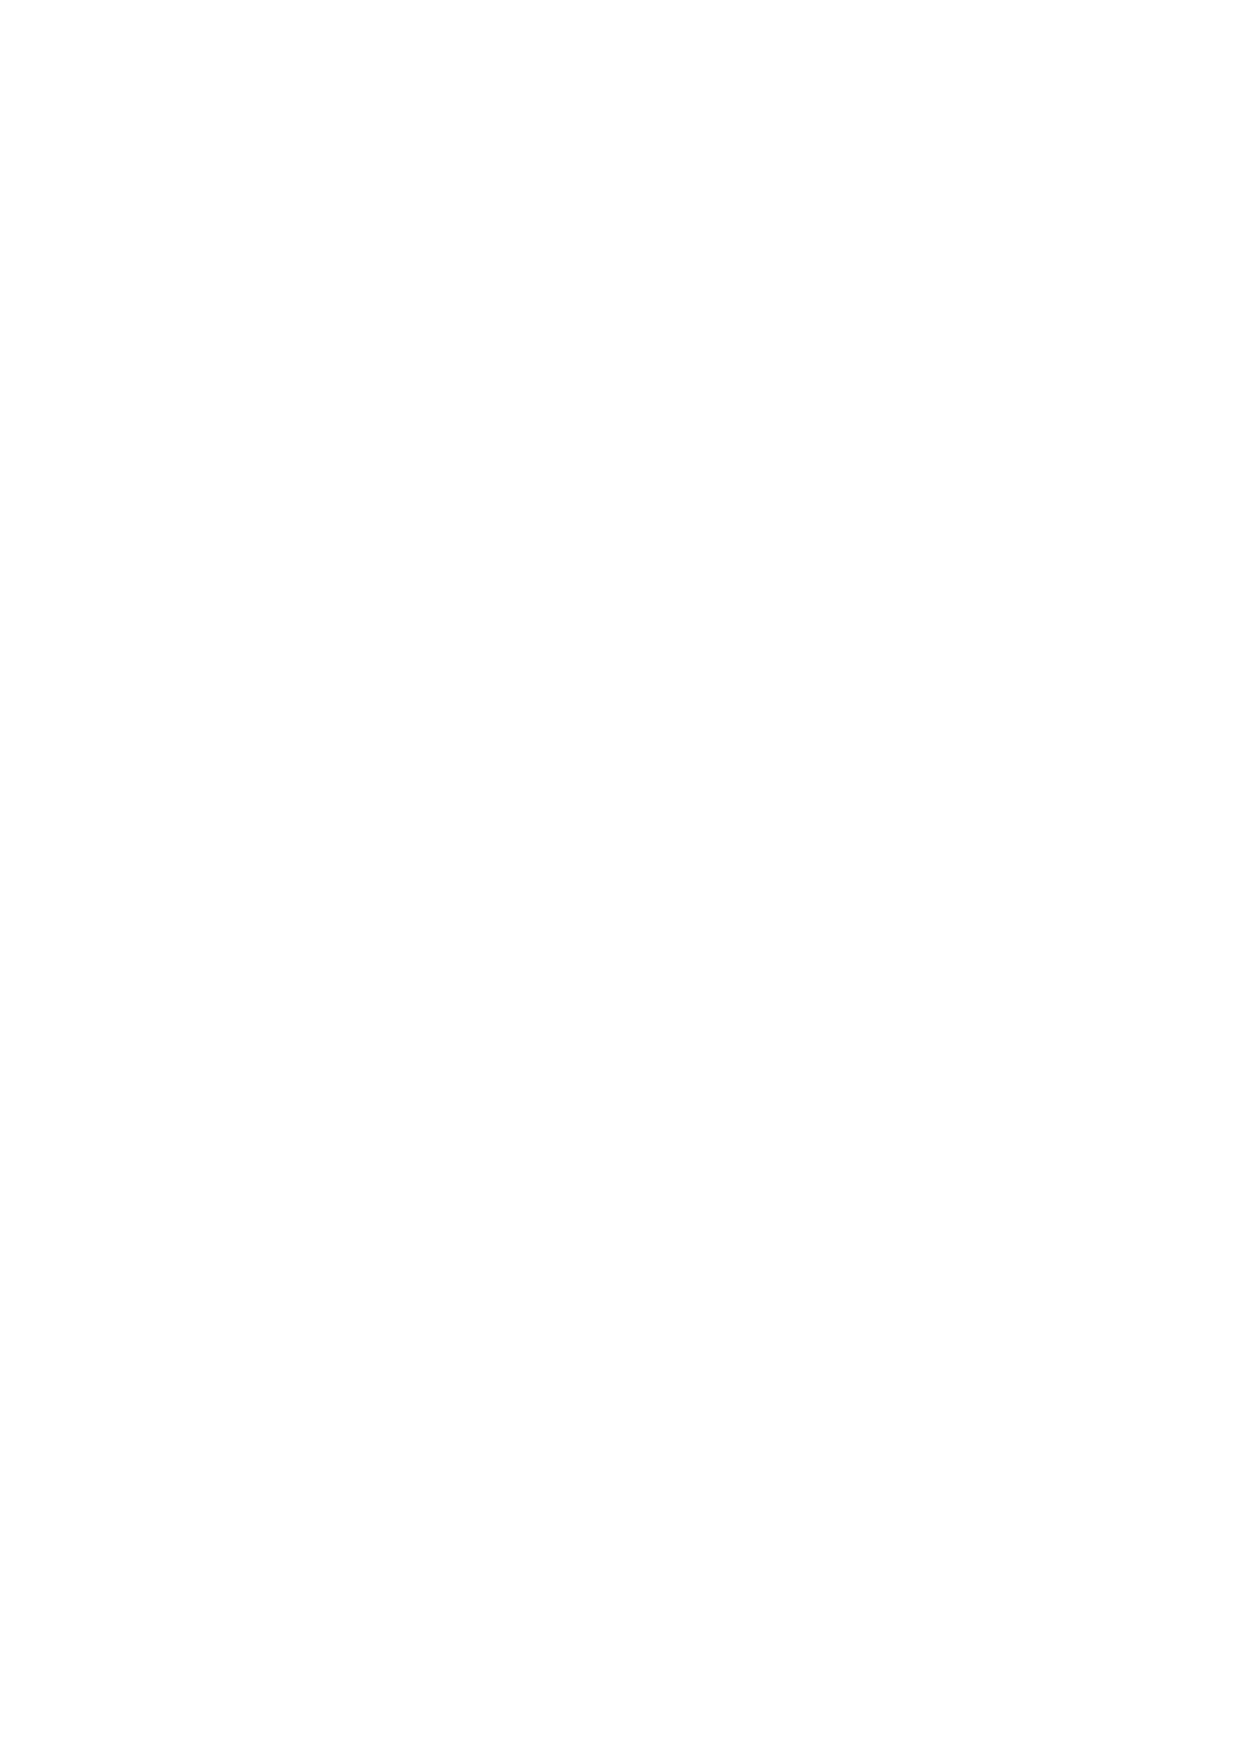
\includegraphics[page=1]{AreaAgg_CaseStudy1_Plot} 
\end{table*}

Recall \sect\ref{sec:AreaAgg_AStar}, for region with 
ID~$i$ we 
define~$k_i$ as the least repetitions that we do to find a 
feasible solution. 
We define the total repetitions 
as~$k_\mathrm{sum}=\sum_{i=1}^\mathcal{N} k_i$, 
where~$\mathcal{N}$ is the number of regions.
After we increased~$M$ to~$400{,}000$, we found optimal 
aggregation sequences for only three more regions, 
but the total repetitions~$k_\mathrm{sum}$ decreased 
quite a bit, from~$102$ to~$89$. 
The numbers of regions that needed certain
overestimation steps are shown in 
\fig\ref{fig:AreaAgg_OverStats}. 
Besides, we visited more arcs and nodes, 
used more time, 
but got (slightly) less cost when $M=400{,}000$.
Although the number of regions 
that needed overestimation is relatively small, 
\Astar spent most of the running time 
on these few regions: $4.4\%$ and $4.0\%$ of the regions 
cost $90.5\%$ and $93.9\%$ of the total running time, 
respectively (see Table~\ref{tab:AreaAgg_CaseStudy1_Statistics}).

\begin{figure}[tb]
	\centering
	\includegraphics[page=2]{AreaAgg_CaseStudy1_Plot}
	\caption{The numbers of regions where our approach was 
		forced to use the given overestimation factors in order 
		to 
		find a solution without exploring more than $M \in 
		\{200{,}000,~400{,}000\}$ nodes of the subdivision 
		graph.}
	\label{fig:AreaAgg_OverStats}
\end{figure}

The details of some regions are presented in 
Table~\ref{tab:CostsInDetail}.
According to the entries with overestimation factor $K_i=0$, 
we often have~$R_\mathrm{type}=1$ and~$R_\mathrm{shape}>1$.
When $K_i=0$, we did not overestimate for region~$i$.
The estimated cost must be smaller or equal to the exact cost,
which results in~$R_\mathrm{type}\ge 1$ 
and~$R_\mathrm{shape}\ge 1$.
$R_\mathrm{type} = 1$ means that our estimation for the 
cost of type change is the best.
A larger~$R_\mathrm{shape}$ means that our estimation for the 
cost of shape is poorer.

\begin{table*}[tb]
	\caption{The costs in detail of some regions, 
		where $M=200{,}000$.  
		Parameters $n$ and $m$ are the numbers of patches and 
		their adjacencies on the start map, respectively.
		Parameter $K$ is the overestimation factor, 
		defined in \sect\ref{sec:AreaAgg_Preliminaries}. 
		We evaluate the quality 
		of our estimations for type change and 
		compactness by listing the numbers~
		$R_\mathrm{type}=g_\mathrm{type}(\Pgoal)
		/h_\mathrm{type}(\Pstart)$ and~
		$R_\mathrm{comp}=g_\mathrm{comp}(\Pgoal)
		/h_\mathrm{comp}(\Pstart)$. \revise{}{Note that if~ 
			$h_\mathrm{type}(\Pstart)=0$, we 
			define~$R_\mathrm{type}=1$.}
	}
	\label{tab:CostsInDetail}
	\centering
	\includegraphics[page=3]{AreaAgg_CaseStudy1_Plot}
\end{table*}


The \Astar algorithm managed to find optimal solutions 
for all the regions with patches fewer than~$15$,
and only found feasible solutions 
for any region with more than~$21$ patches
(see \tab\ref{tab:CostsInDetail}).
In the~$702$ regions that \Astar solved to optimality,
the greedy algorithm failed to find optimal solutions for~$295$
regions.
The greedy algorithm cost as much as $41.7\%$ more than \Astar; 
for region~$85$, the greedy algorithm cost~$0.777$, while 
\Astar cost~$0.548$
(see \fig\ref{fig:AreaAgg_CaseStudy1_Rg85}).
As the patches in the two sequences are the same,
the two results have the same cost of compactness.
The major difference is the choice of the first step, 
from~$8$ patches to~$7$.
When aggregating the smallest patch on the start map
with the surrounding patch,
our greedy algorithm chooses the type 
which is closer to the goal type.
In this case, the smallest patch has type~$5112$, and the 
surrounding one has~$2112$.
The type of the goal map is~$4102$.
According to \fig\ref{fig:AreaAgg_TypeDistances},
type distance~$d(5112,4102)=4$ and~$d(2112,4102)=6$.
As a result, our greedy algorithm use~$5102$ as the type for the 
new patch. 
This choice is a big mistake because the largest patch on the 
start map is assigned type~$5112$ and later the target type, 
$4102$.
These assignment cost more than the sequence obtained from 
\Astar, where the largest patch on the start map is changed to 
the target type directly.

In the $32$~regions that 
\Astar failed to find optimal aggregation sequences,
the greedy algorithm found solutions better than \Astar 
for~$15$ regions ($46.9\%$).
%
The greedy algorithm cost $15.9\%$ less than \Astar at most; 
for region~$543$, the greedy algorithm cost~$0.112$, while 
\Astar using overestimation parameter~$K=7$ cost~$0.134$
(marked in \tab\ref{tab:CostsInDetail}).
\fig\ref{fig:AreaAgg_CaseStudy1_Rg543} shows 
some intermediate results obtained by
\Astar and the greedy algorithm.
Interestingly, the two methods produced the same sequence until 
there were~$8$ patches left.
Then due to the overestimation, \Astar did some bad moves
because the bad aggregation sequence still seemed better 
than other sequences.
In contrast, the greedy algorithm was looking for locally good 
aggregation options.
%
The greedy algorithm cost at most $17.4\%$ more than \Astar; 
for region~$155$, the greedy algorithm cost~$0.372$, while 
\Astar cost~$0.317$
(marked in \tab\ref{tab:CostsInDetail}).



\begin{figure}[tb]
	\centering
	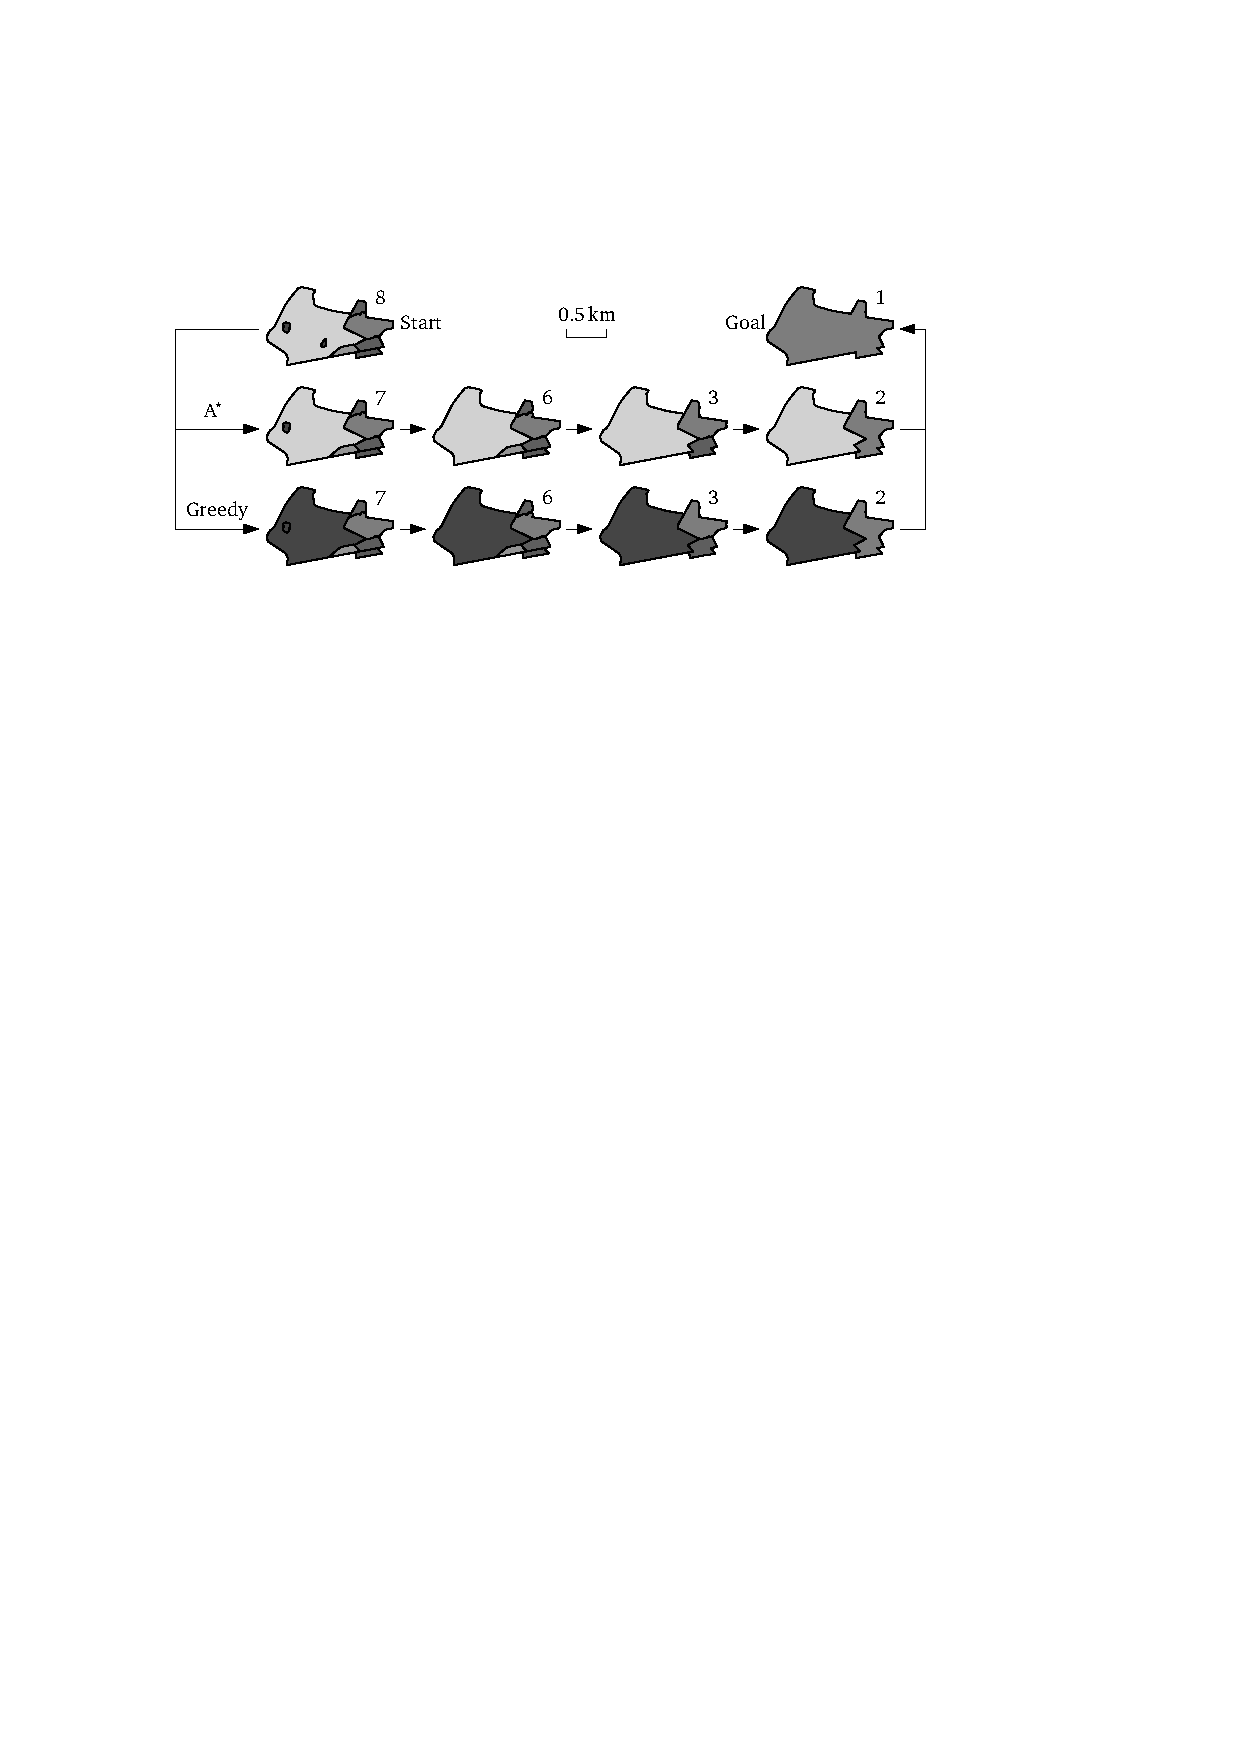
\includegraphics[page=1]{AreaAgg_CaseStudy1}
	\caption{Aggregation sequences of region~$85$ 
		obtained by \Astar and the greedy algorithm.
		The numbers of the patches are shown in the figure.
		In order to save space, we did not show the results when 
		there are~$4$, $5$, and~$6$ patches, 
		which one can easily deduce.}
	\label{fig:AreaAgg_CaseStudy1_Rg85}
\end{figure}

\begin{figure}[tb]
	\centering
	\includegraphics[page=2]{AreaAgg_CaseStudy1}
	\caption{Some intermediate subdivisions of region~$543$ 
		obtained by \Astar and the greedy algorithm.
		The numbers of the patches are shown in the figure.
		In the sequence obtained by \Astar, 
		a pair of circles or a pair of squares indicates that
		the two parts are actually in the same patch.
	}
	\label{fig:AreaAgg_CaseStudy1_Rg543}
\end{figure}

Finally, an optimal aggregation sequence of region~$53$
(marked in \tab\ref{tab:CostsInDetail})
is shown in \fig\ref{fig:AreaAgg_CaseStudy1_Rg53}.

\begin{figure}[tb]
	\centering
	\includegraphics[page=3]{AreaAgg_CaseStudy1}
	\caption{Some intermediate subdivisions of region~$53$ 
		obtained by \Astar.
		The numbers of the patches are shown in the figure.
	}
	\label{fig:AreaAgg_CaseStudy1_Rg53}
\end{figure}


%\todo[inline]{It turned out that the objective function $g$ 
%seems rather robust
%	against changes of~$\lambda$.  For region~77, we 
%	varied~$\lambda$ in
%	the range $\{0.1,0.5,0.9\}$, but the resulting aggregation 
%	sequences
%	stayed almost the same.  When we used even larger 
%	values 
%	for~$\lambda$ (e.g.,~$0.99$), the (good) influence of type 
%	change was mitigated 
%	and, as a
%	result, we needed to overestimate (with factor~$K=8$).}



\subsection{Using costs of type change and length}
We compare greedy algorithm, \Astar, and our ILP
using $g_2(\Pnode)$,
which is a combination of the costs 
of type change and length (see \eq\ref{eq:g_2}).
For \Astar, we overestimated 
whenever we could not find a solution after 
having visited~$M=200{,}000$ nodes (see 
Sec.~\ref{sec:AreaAgg_AStar}).
The most time-consuming instance for \Astar was region~$94$,
which took~$160.0\,$s to find a feasible solution 
with overestimation factor~$K=31$.
To void waiting too long for our ILP,
we set the time limit as $160\,$s.
If our ILP cannot find an optimal solution 
in this amount of time, a feasible solution may be returned.
For some instances, our ILP cannot even 
find a feasible solution.

Similar to \tab\ref{tab:AreaAgg_CaseStudy1_Statistics},
we present some statistics in \tab\ref{tab:AreaAgg_CaseStudy2_Statistics}.
\Astar found optimal solutions for~$695$ of the~$734$ regions.
Again, it spent most of the running time 
on the few regions that needed 
overestimations:~$5.3\%$ of the regions 
cost~$89.5\%$ of the total running time.
Overall, \Astar cost~$438.2$, which is~$3.9\%$ 
less than the cost of the greedy algorithm ($455.8$).

\Astar managed to find optimal solutions 
for all the regions with patches fewer than~$15$, and 
only found feasible solutions for any region 
with more than~$21$ patches.
%
In the~$39$ regions that \Astar failed to find optimal solutions,
the greedy algorithm found solutions better than \Astar 
for~$25$ regions~($64.1\%$), 
which is more than~$46.9\%$ in the first experiment.
%
The ILP managed to find optimal solutions 
for all the regions with patches fewer than~$8$,
and failed to find optimal solutions
for any region with more than $8$ patches.
In the~$39$ regions that \Astar failed to find optimal solutions,
ILP did not even find feasible solutions for any of them.
Our ILP found optimal solutions for~$441$ regions,
and found feasible solutions for~$73$ regions.

\begin{table*}[tb]
	%\small	
	\centering
	\caption{A comparison of Greedy and \Astar		
		when using cost function~$g_2$.
		The notations are the same as 
		\tab\ref{tab:AreaAgg_CaseStudy1_Statistics}.
		%
		Symbols~$g_\mathrm{t}$, $g_\mathrm{l}$, and~$g_2$
		denote the sums of~$g_\mathrm{type}(\Pgoal)$,
		$g_\mathrm{length}(\Pgoal)$, and~$g_2(\Pgoal)$,
		respectively, over all instances (see 
		\eqs\ref{eq:g_type}, \ref{eq:g_length}, 
		and~\ref{eq:g_2}).
	}
	\label{tab:AreaAgg_CaseStudy2_Statistics}
	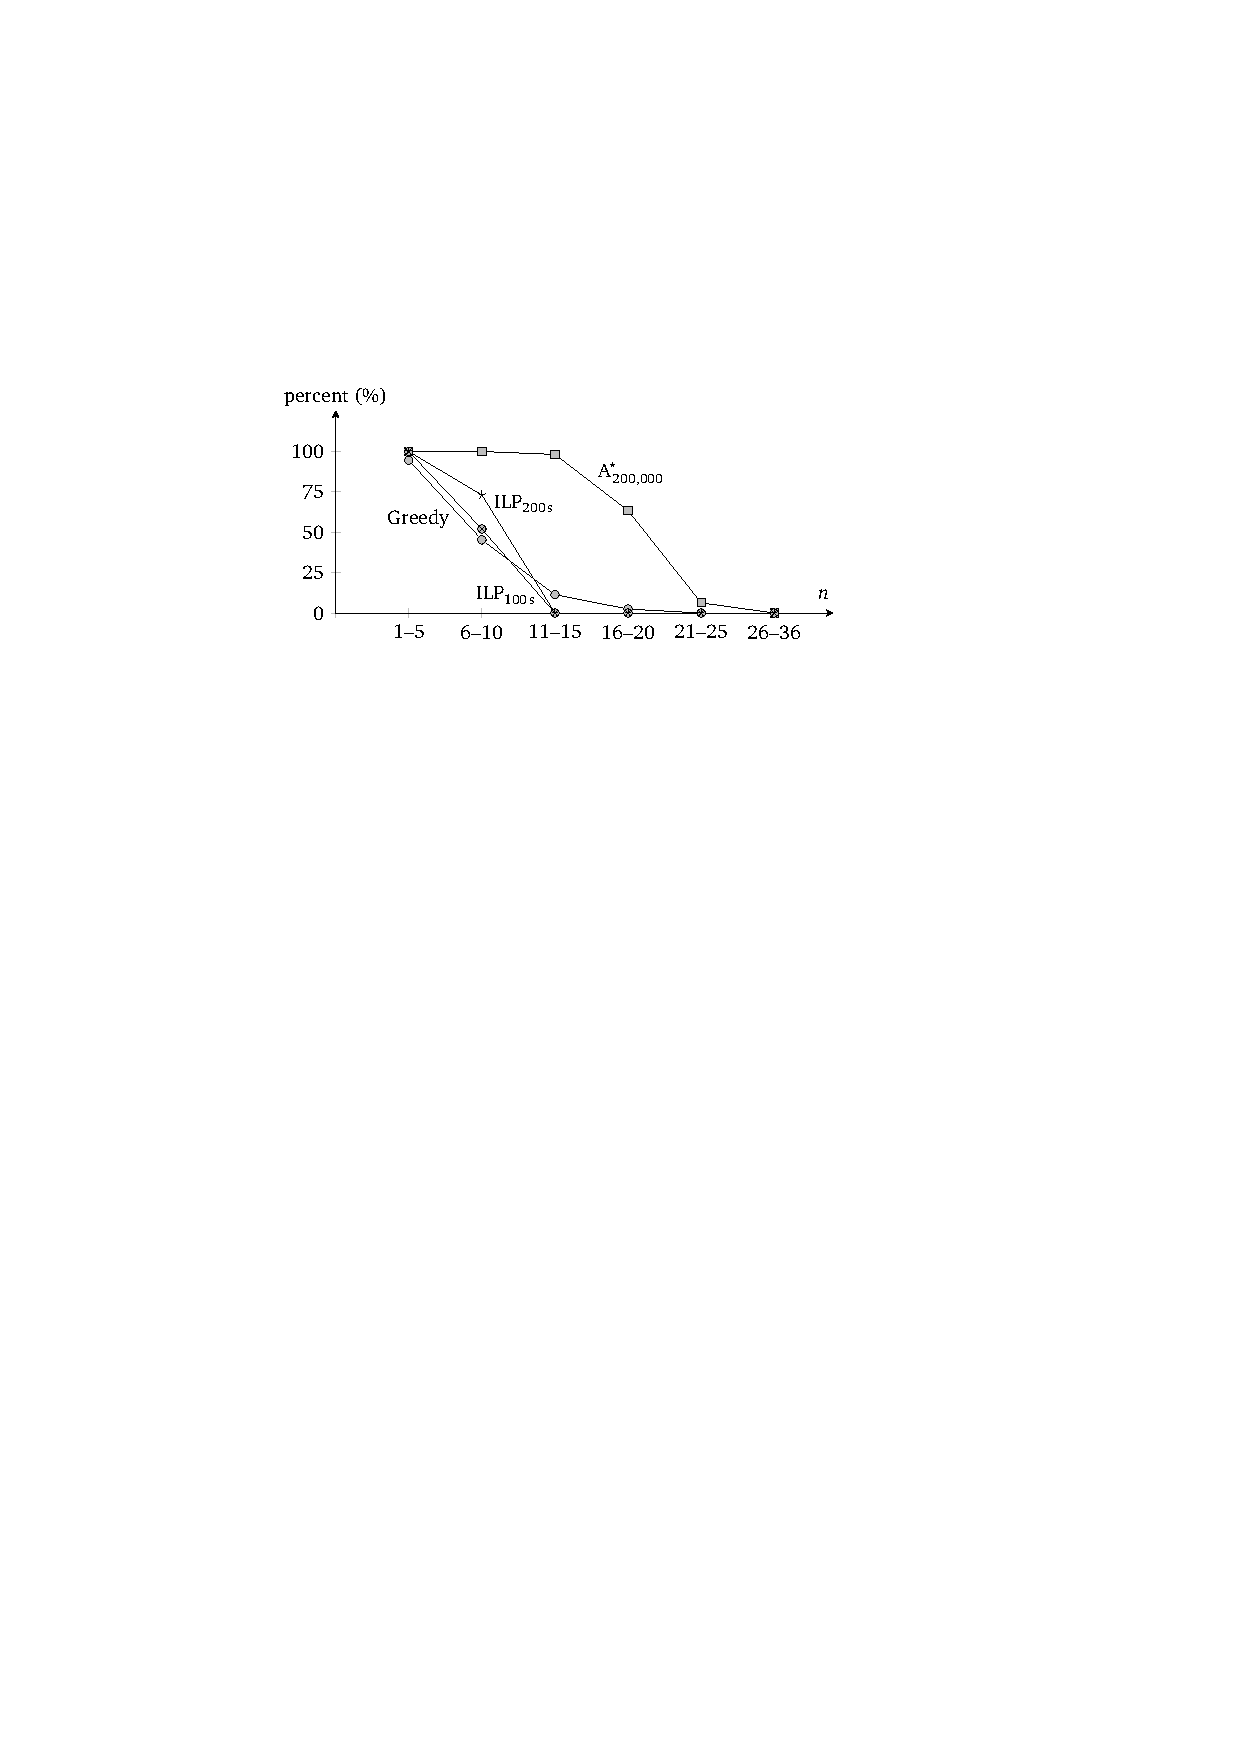
\includegraphics[page=1]{AreaAgg_CaseStudy2_Plot} 
\end{table*}



Among all the instances that were solved to optimality
in both experiments,
region~$358$
(marked in \tab\ref{tab:CostsInDetail})
is the largest one.
In both experiments, the cost of type is~$0.044$.
We show the optimal sequences respectively obtained 
by using costs~$g_1$ and~$g_2$ in
\fig\ref{fig:AreaAgg_CaseStudy2_Rg358}.
We, however, noticed some unpleasant aggregations.
The step from~$8$ patches to~$7$ patches 
when using cost function~$g_1$ is a bad move.
In stead we expect the result of \fig\ref{fig:AreaAgg_CaseStudy2_Rg358}a.
Also in the step but using cost function~$g_2$,
we expect the result of
\fig\ref{fig:AreaAgg_CaseStudy2_Rg358}b.

\begin{figure}[tb]
	\centering
	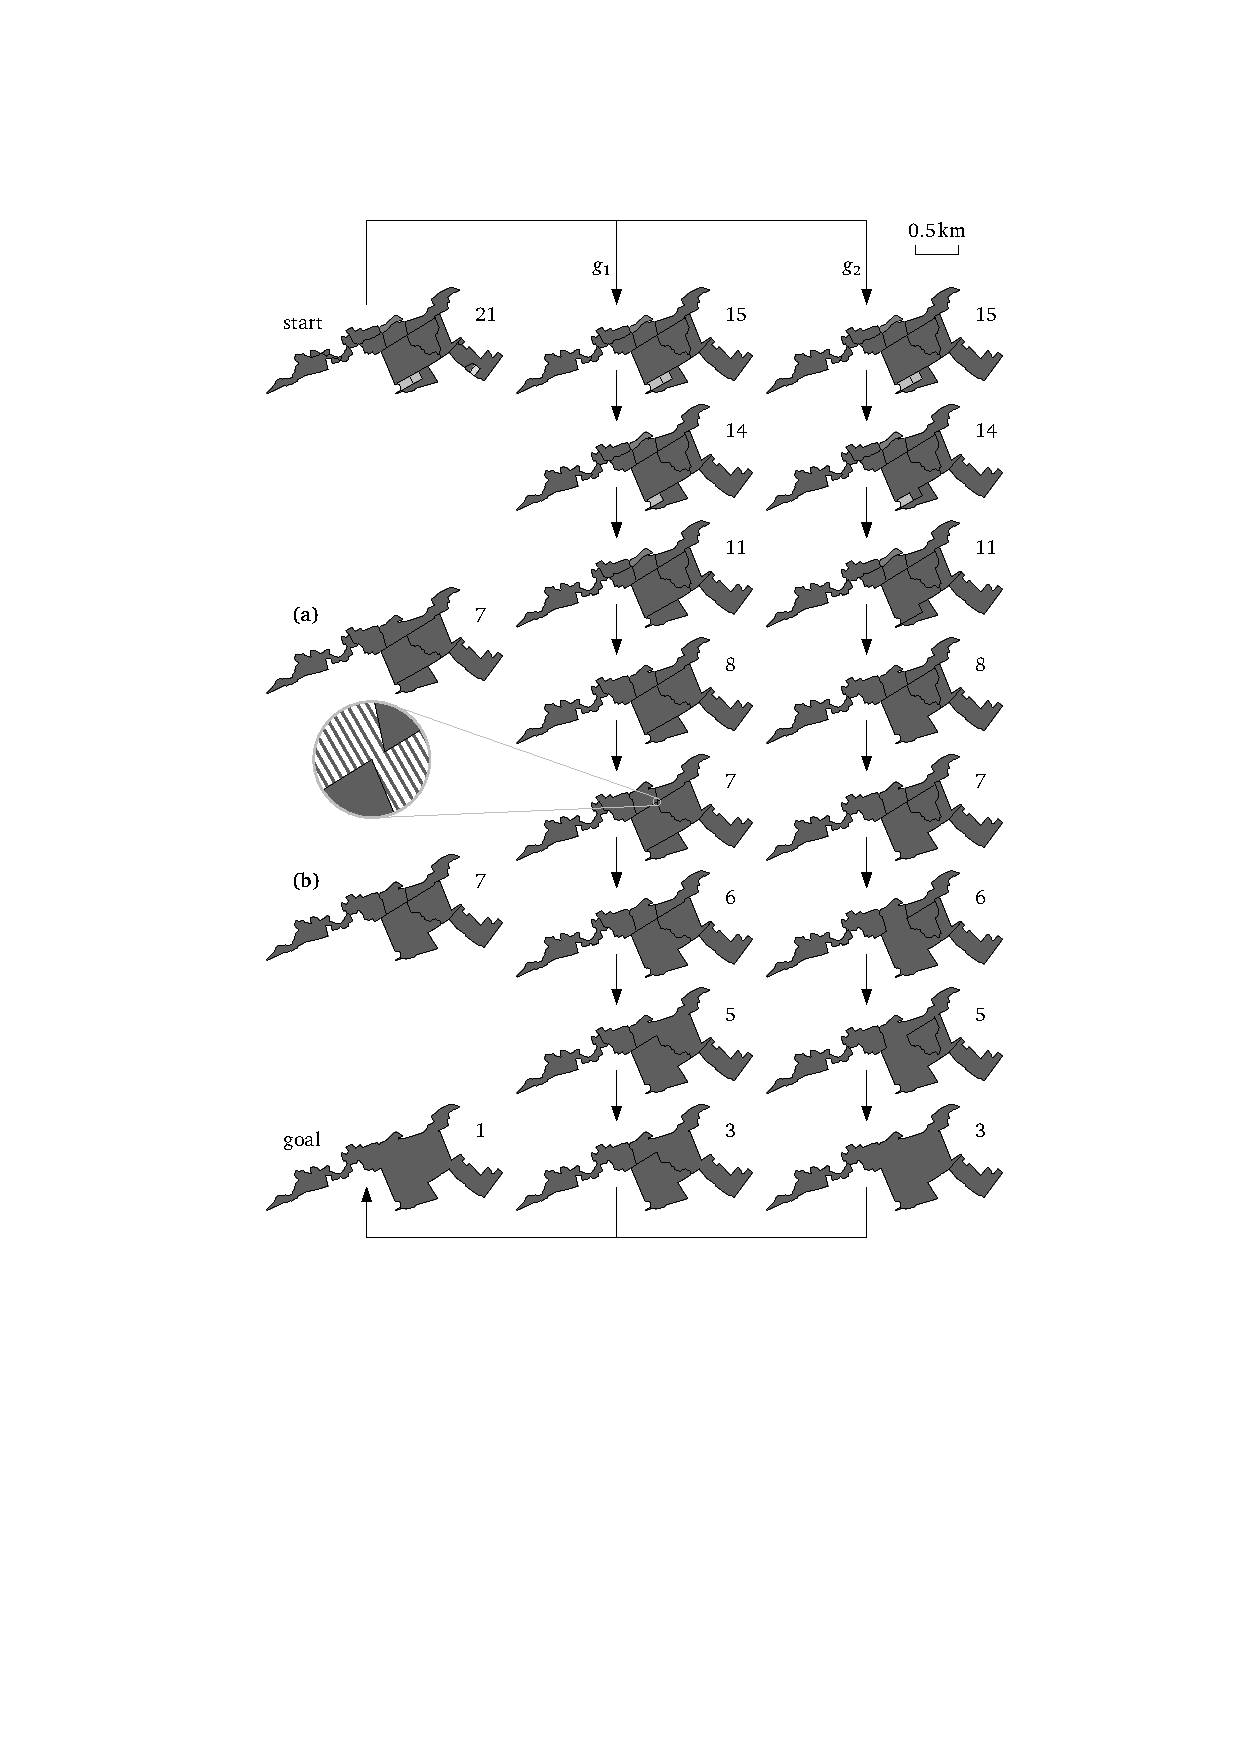
\includegraphics[page=1]{AreaAgg_CaseStudy2}
	\caption{Some intermediate subdivisions of region~$358$ 
		obtained by \Astar with different cost functions.
		The numbers of the patches are shown in the figure.
	}
	\label{fig:AreaAgg_CaseStudy2_Rg358}
\end{figure}


\section{Concluding Remarks}
\label{sec:AreaAgg_Conclusions}
In this chapter, we investigated the problem of 
finding optimal sequences for area aggregation.
We compared three methods to solve this problem, namely, 
a greedy algorithm, \Astar, and an ILP-based algorithm.
The greedy algorithm is used as a benchmark.
Unsurprisingly, it run faster than the other two methods by far.
According to our experiments, \Astar found area aggregation sequences
with the least cost overall regions.
For some instances, however, \Astar had to overestimate
in order to find feasible solutions.
The ILP-based algorithm finds optimal solutions for some regions,
but it sometimes cannot even find a feasible solution.


For \Astar we have a good estimation for the cost of type change, which helps a lot to reduce the search space. 
our estimation for the cost of shape (compactness or length) is poor.
There are two ways to improve our \Astar.
First, during the searching we can forget a node, of the graph,
if all the neighbors of this node have been visited.
By testing a case, we learned that half of the nodes can be 
forgotten during the pathfinding process.
In this way, we can release some main memory and visit more nodes
provided that our main memory is limited.
Once we arrive at the goal, we know the cost for an optimal solution
(the least cost).
As many nodes have been forgotten, we do not have the shortest path so far.
We have to run \Astar again.
In this time we know for sure that 
a path is not optimal 
if it costs more than the least cost.
We can prune more branches in order to save main memory.
As a result, we are more likely to find optimal solutions
when the main memory is limited.
Second, if we obtain a solution based on overestimation, 
then we know the cost of this non-optimal solution.
We may reduce the overestimation factor by pruning the branches
that cost more than the non-optimal solution.

For the ILP-based algorithm, we can add more constraints to
reduce the choices of variables.
For example, it is easy to see that 
if polygons~$p$ and~$q$ are both assigned to center~$r$,
then polygons~$q$ and~$p$ are also assigned to center~$r$,
and vice versa.
Hence, there always holds
\begin{equation}
\label{eq:CstrZX}
z_{t,p,q,r}= z_{t,p,q,r} \qquad
\forall t \in {T} \setminus \{1,n\}, 
\forall p, q, r \in P. \nonumber
\end{equation}
Whether or not adding such kinds of constraints 
will speed up our ILP
needs to be tested.
Although inter linear programming may be not good at 
finding optimal sequences for area aggregation, 
problems are easy to be formulated as an ILP.
As stated by \citet[p.~861]{Cormen2009}, 
"an efficient algorithm designed specifically for a problem 
will often be more efficient than 
linear programming both in theory and in practice. 
The real power of linear programming comes from 
the ability to solve new problems."

In our experiment, we see that 
we have unpleasant intermediate results
even when a sequence is optimal.
This means that we may need model our problem in a better way,
for example, by using other cost functions.

A requirement for the aggregation is to keep 
important land-cover areas (such as a settlement surrounded by 
farmlands) longer. 
%
Another requirement is that 
aggregating two areas and 
getting an area with a generalized type. 
For example, aggregating 
farmland with hedge yields an area with type vegetation.
%
These issues can be considered in our future work.
%









